\documentclass[14pt, table]{extarticle}
\usepackage{amsfonts}
\usepackage{amsmath}
\usepackage[utf8]{inputenc}
\usepackage[a4paper, total={7in, 10.5in}]{geometry}
\usepackage[table]{xcolor}
\usepackage{tgbonum}
\usepackage{float}
\usepackage{graphicx}
\graphicspath{ {./images/} }
\DeclareGraphicsExtensions{.png,.jpg}
\usepackage{caption}
\usepackage{tikz}
\usepackage{circuitikz}
\usepackage[T1]{fontenc}
\usetikzlibrary{quotes,angles}
\usetikzlibrary{arrows}
\usetikzlibrary{circuits.logic.US}
\usetikzlibrary{positioning}
\hyphenpenalty 500
\usepackage{subfig}
\usepackage{array}

\title{\textbf{Sprawozdanie} \\ \Large{Ćwiczenie 6}}
\date{Data wykonania: 7 czerwca 2023}
\author{ \Large{Jan Kwinta, grupa 12} \\ \large{Prowadzący ćwiczenia: dr. Szymon Niedźwiedzki}}

\newcommand{\nl}{\vspace{0.5cm}}
\newcommand{\nz}{\vspace{1.5cm}}

\begin{document}
\maketitle

\paragraph{Wstęp \\}

Na szóstych i ostatnich laboratoriach z elektroniki cyfrowej zajmowaliśmy się przetwornikami analogowo-cyfrowymi. Są to układy, które operując zarówno analogowymi wartościami (np. wartość napięcia) oraz cyfrowymi (zapis binarny) i służą do powiązania (konwersji) jednego systemu przesyłu wartości z drugim. Przetworniki A/C znajdują liczne zastosowania w dziedzinie przesyłu informacji — to one stanowią łącznik pomiędzy cyfrowymi, wydajnymi komputerami a światem czujników i sensorów, a więc wartości przeważnie ciągłych, mierzonych w sposób analogowy. \\

Przetworniki A/C stosuje się do przetwarzania napięć stałych, jak również napięć zmieniających się w czasie. Przetwarzanie A/C tworzą 3 etapy: próbkowanie, kwantyzacja i kodowanie. Pobieranie i przetwarzanie próbek napięcia odbywa się w zadanych chwilach czasu, na ogół okresowo z pewną częstotliwością, zwaną częstotliwością próbkowania. Aby dobrze dobrać częstotliwość próbkowania i uniknąć tzw. \textit{aliasingu} stosuje się twierdzenie Nyquista-Shannona, nazywane też twierdzeniem o próbkowaniu: "Jeśli sygnał ciągły nie ma składowych widma o częstotliwości równej lub większej niż B, może on zostać jednoznacznie odtworzony z ciągu jego próbek tworzących sygnał dyskretny, o ile próbki te zostały pobrane z częstotliwością co najmniej 2B." Oznacza to w praktyce, że ustalając częstotliwość próbkowania powinniśmy uczynić ją przynajmniej 2 razy większą niż najwyższa występująca w przetwarzanym sygnale składowa widma. \\

Kwantyzacja sygnału polega na zmniejszeniu precyzji pobranych wartości w momencie próbkowania. Każda wartość wejściowa wypadająca w określonym przedziale jest w wyniku kwantyzacji odwzorowana na jedną wartość wyjściową przypisaną temu przedziałowi, czyli tak zwany poziom reprezentacji. To właśnie ilość poziomów reprezentacji przekłada się na rozdzielczość przetwornika — liczbę dyskretnych wartości jakie może on wytworzyć. Zwykle wyraża się ją w bitach. Przykładowo, przetwornik A/C, który potrafi przetworzyć próbkę sygnału na jedną z 256 wartości liczbowych posiada rozdzielczość równą 8 bitów, ponieważ $2^{8}=256$. Kodowanie polega na przyporządkowaniu danemu poziomowi reprezentacji liczby w systemie binarnym, która może być potem odczytana przez układ cyfrowy. \\

Przetworniki cyfrowo-analogowe to urządzenia działające w dokładnie odwrotny sposób. Przetwarzają one sygnał cyfrowy na sygnał analogowy w postaci prądu elektrycznego lub napięcia o wartości zależnej od wejściowego sygnału cyfrowego.

\paragraph{Zadanie 3. \\}

\textbf{3.1} Zapoznanie się z budową i działaniem modułów przetwornika A/C typu FLASH: 
\begin{itemize}
	\item[a)] modułu komparatorów, 
	\item[b)] transkodera RPP-S (Ręcznie Programowana Pamięć Stała),
	\item[c)] transkodera RPP-SRAM (Ręcznie Programowana Pamięć SRAM).
\end{itemize}

\begin{figure}[H]
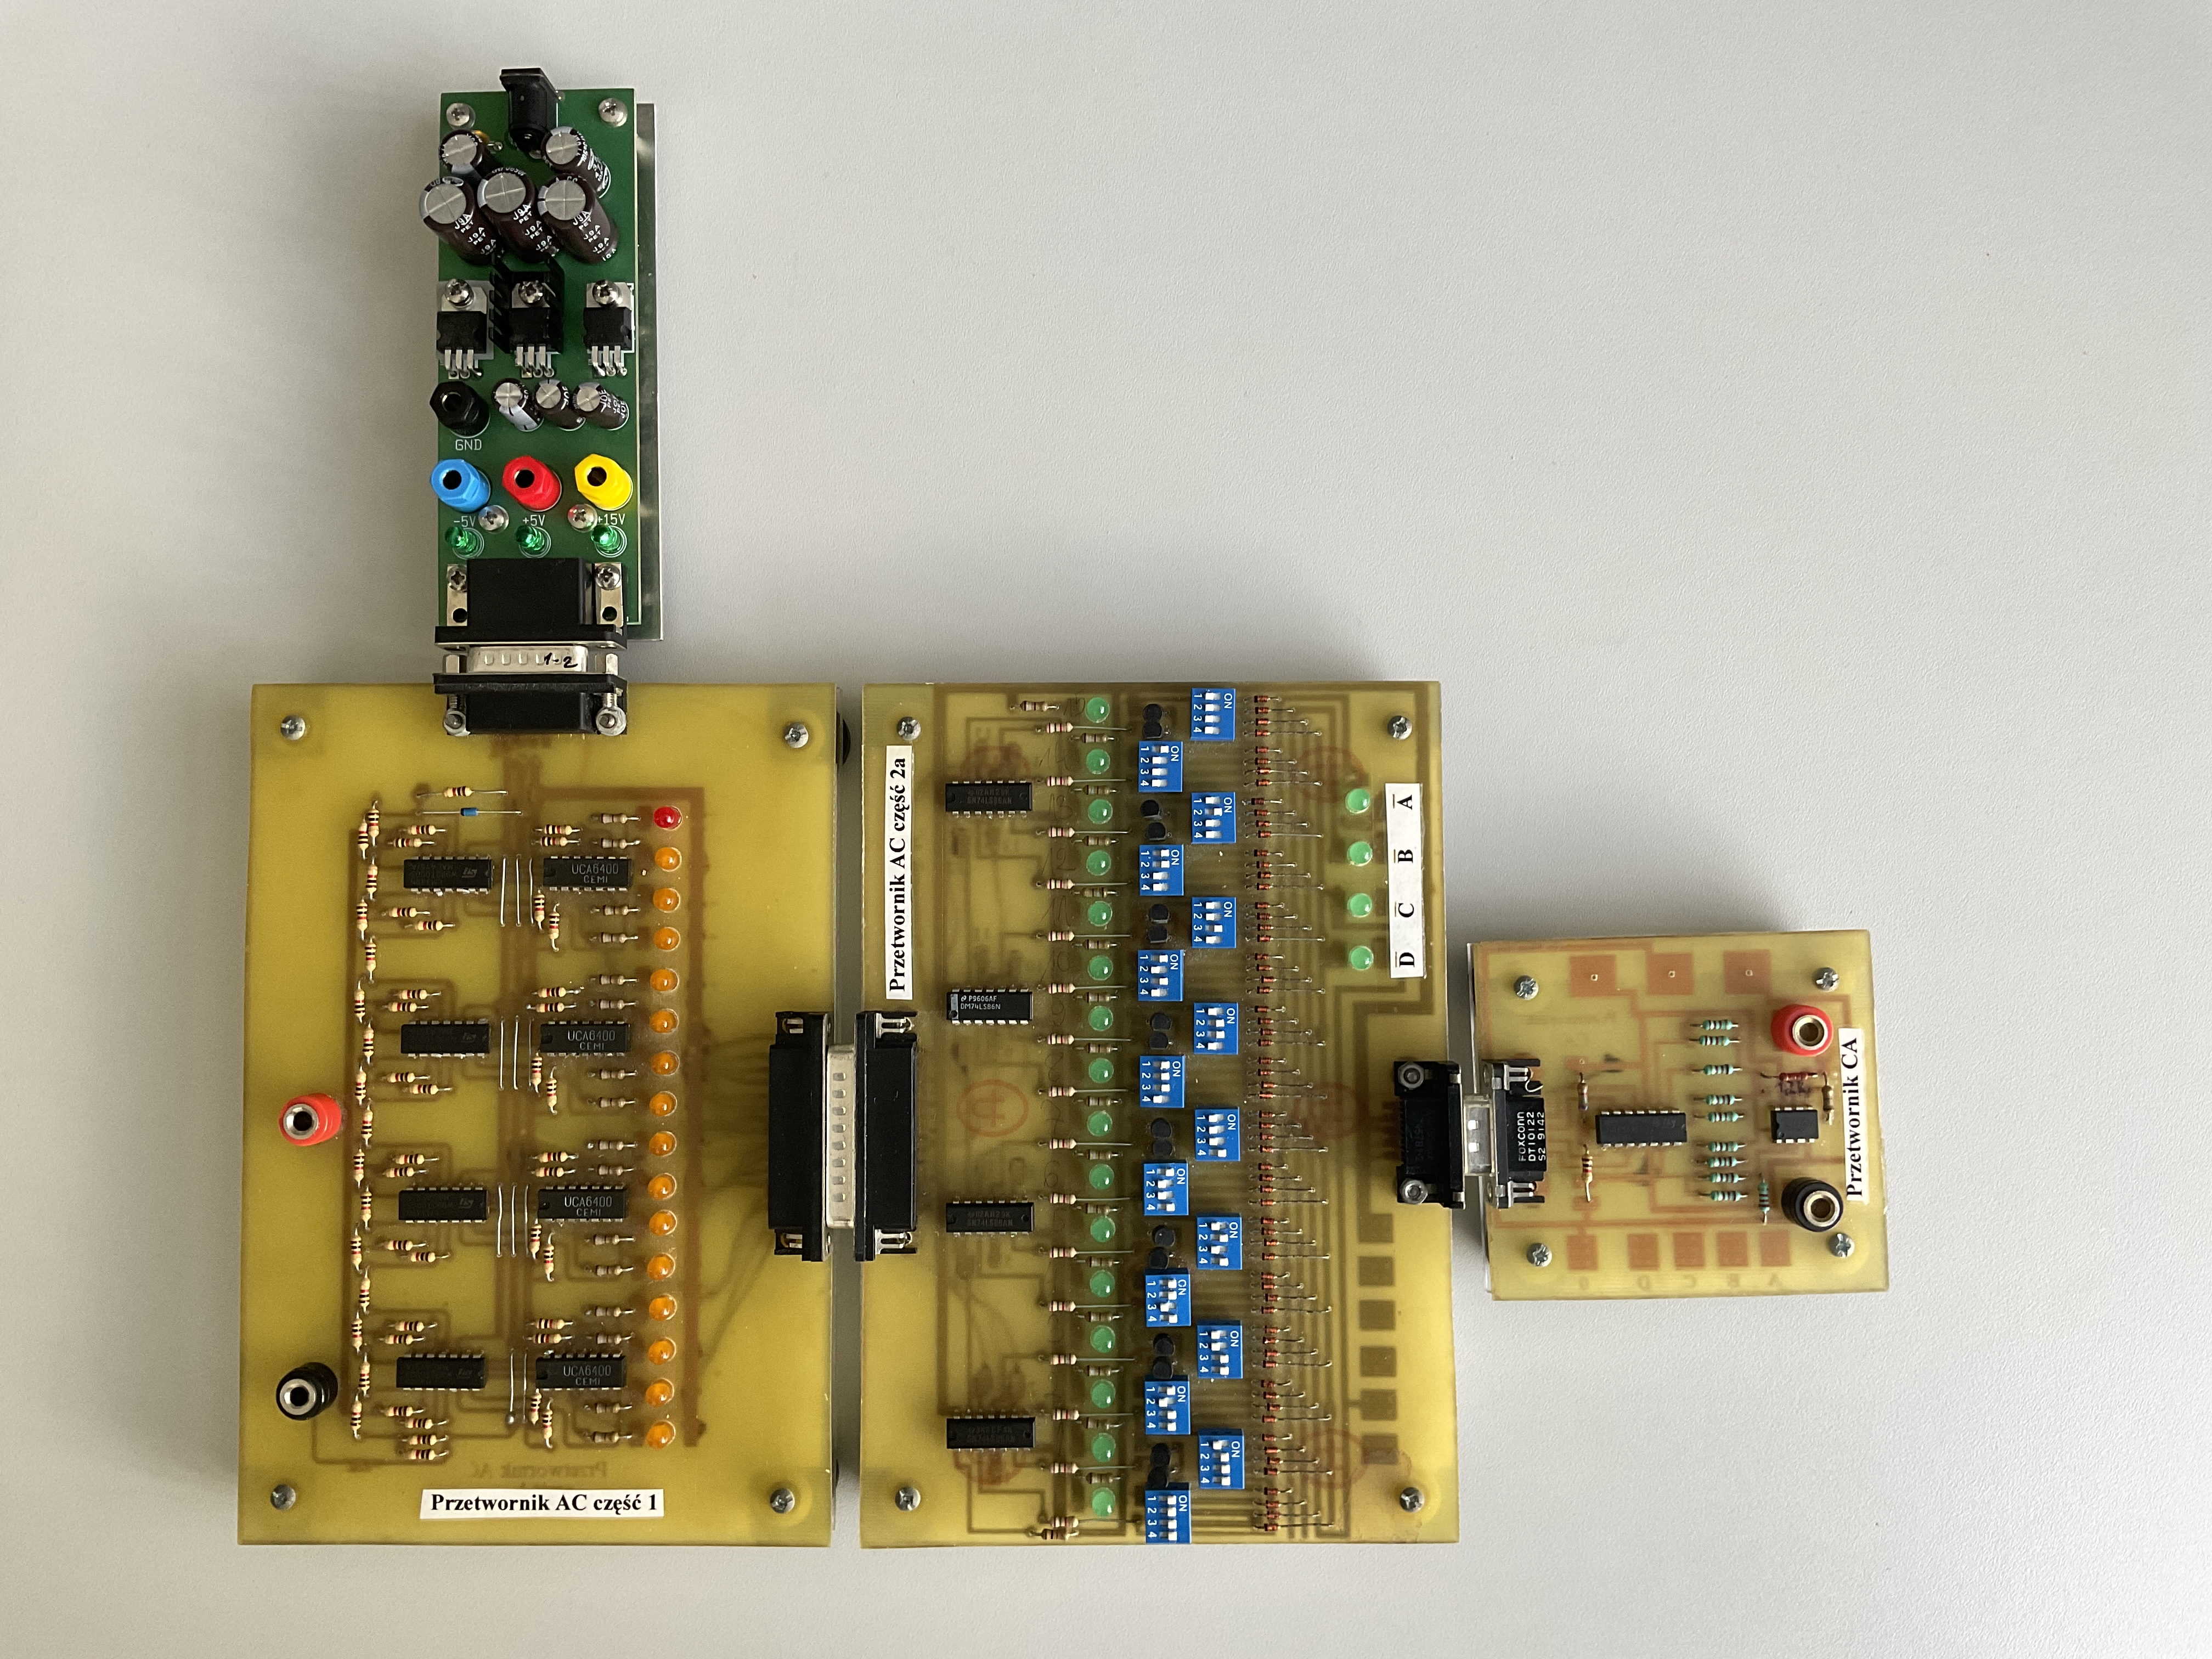
\includegraphics[width=8cm]{C0}
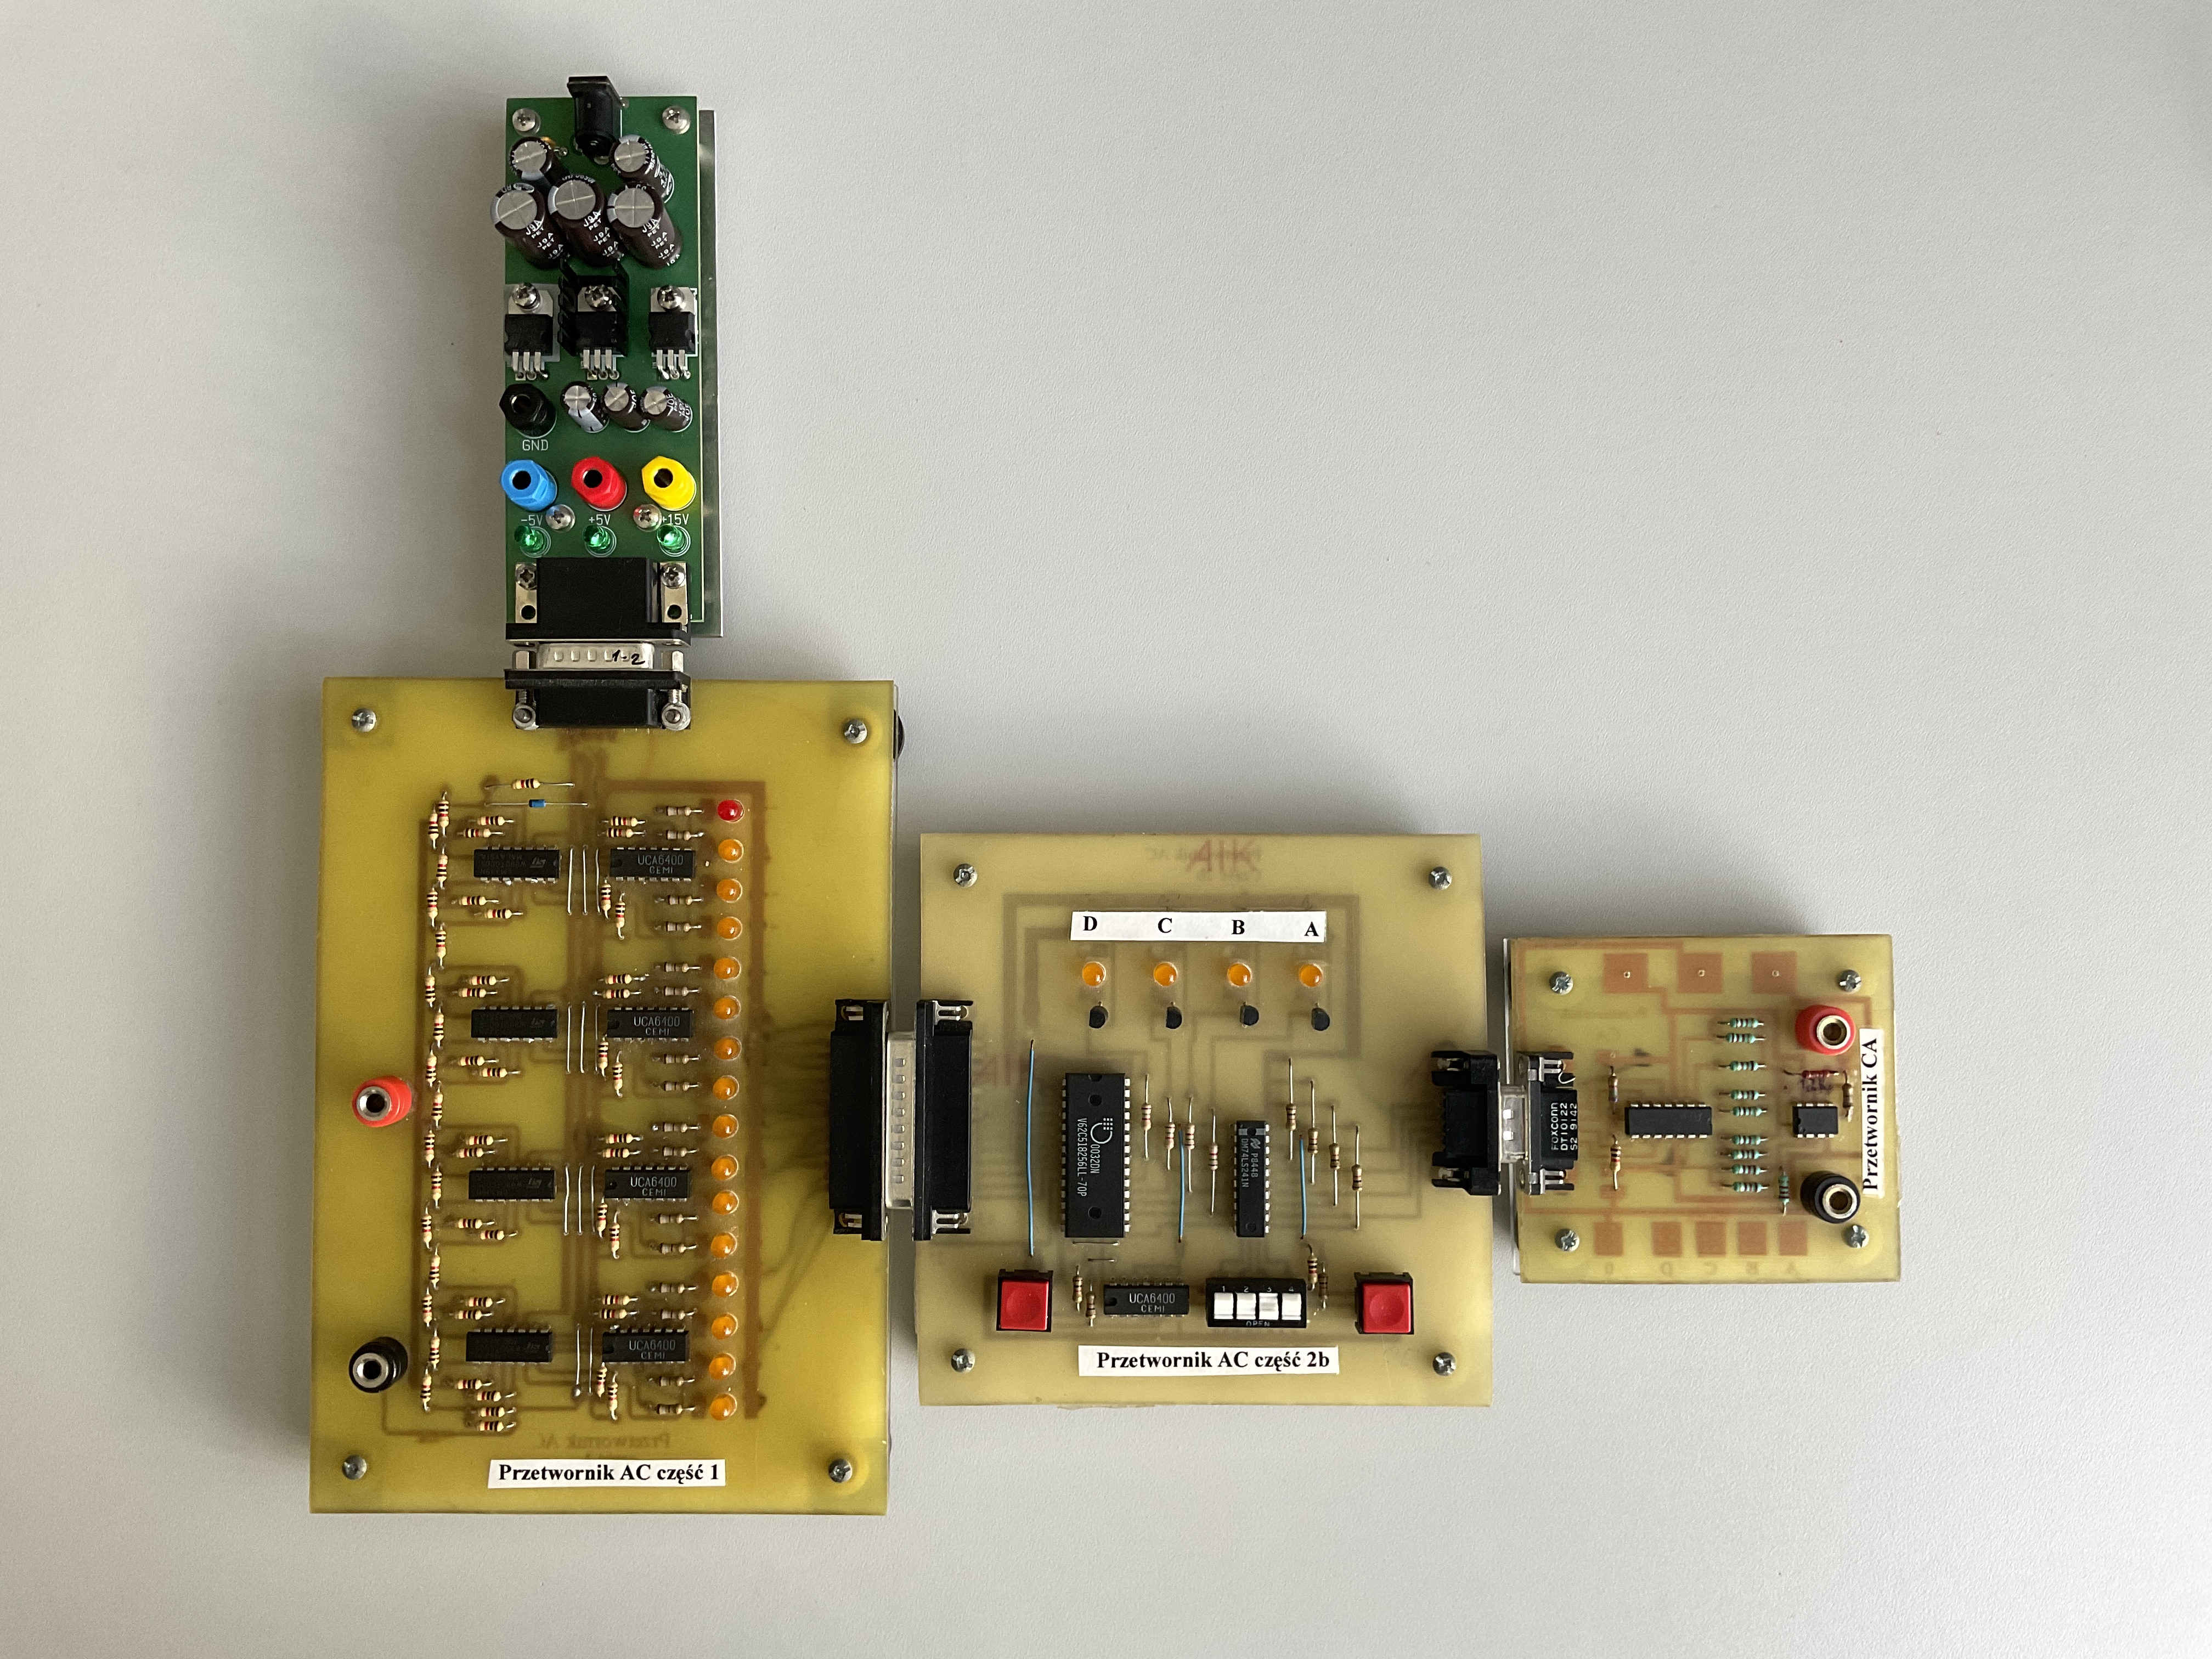
\includegraphics[width=8cm]{C3}
\centering
\captionsetup{labelformat=empty}
\caption{Zdjęcia 1 i 2: Moduł komparatorów połączony z transkoderem RPP-S (lewe zdjęcie) i transkoderem RPP-SRAM (prawe zdjęcie).}
\end{figure}

\begin{figure}[H]
\includegraphics[width=10cm]{D0}
\centering
\captionsetup{labelformat=empty}
\caption{Schemat 1: Schemat ideowy modułu komparatorów.}
\end{figure}

Zadaniem modułu komparatorów jest jest pobranie sygnału analogowego w postaci napięcia i wstępne jego przetworzenie. Główny element funkcyjny tego bloku stanowi szesnaście komparatorów oraz drabinka rezystorowa. Układ ten posiada 15 wyjść, których stany sygnalizowane są diodami LED. Działanie układu polega na załączaniu kolejnych wyjść w miarę wzrostu napięcia wejściowego, to jest: im wyższe napięcie wejściowe tym większa wyjść ma stan logiczny prawda. Napięcie wejściowe powinno zawierać się w zakresie od $0$ do $10 \ V$. Na wyjściu układu wynik reprezentowany jest przez kod składający się z ciągu logicznych jedynek i zer. Ilość ustawionych jedynek reprezentuje wartość napięcia podawanego do przetwornika. Napięciu wejściowemu $0 / V$ odpowiada brak aktywnych linii wyjściowych, natomiast w miarę wzrostu napięcia wejściowego kolejne linie wyjściowe przechodzą w wysoki stan logiczny. Powyżej poziomu $10 / V$ aktywne są wszystkie wyjścia, a ponadto zapala się dioda sygnalizująca przekroczenie zakresu (przesterowanie). \\

\begin{figure}[H]
\includegraphics[width=8cm]{D1}
\includegraphics[width=8cm]{D2}
\centering
\captionsetup{labelformat=empty}
\caption{Schematy 2 i 3: Schematy ideowe odpowiednio transkodera RPP-S i transkodera RPP-SRAM.}
\end{figure}

Zadanie modułów transkoderów jest identyczne, ale zasada ich działania jest różna. Obydwa te układy przyjmują na wejściu "kod linijkowy" z wyjścia modułu komparatorów i przetwarzają go na naturalny kod binarny. Moduł RPP-S Posiada szereg bramek XOR, które przekształcają sygnał z wejścia na kod "1 z 16", czyli ze wszystkich szesnastu bitów zapalony jest ten, który odpowiada najbardziej znaczącemu bitowi, który jest aktywny na wejściu. Możemy następnie ustawić, ręcznie przestawiając przełączniki, jaki bit z sygnału "1 z 16" odpowiada liczbie w naturalnym kodzie binarnym na wyjściu. Moduł RPP-SRAM jest pamięcią ulotną. Moduł ten posiada scalony układ pamięci stanowiący rejestr, do którego komórek adresowych można odwołać się poprzez 15 linii wejściowych. Zatem dwa różne sygnały wyjściowe z modułu komparatorów odpowiadają różnym komórkom w pamięci transkodera. Aby zaprogramować co ma się znaleźć w tych komórkach należy podać odpowiedni adres na wejście, ustawić żądaną wartość za pomocą przełączników a następnie nacisnąć przyciski Output Enable i Write Enable.

\newpage
\textbf{3.2, 3.3} Programowanie transkodera RPP-S.u Połączenie moduł komparatorów z transkoderem RPP-S. Na wejście modułu komparatora podanie regulowanego napięcie stałego. Zmieniając poziom napięcia wejściowego zaprogramowanie transkodera w ten sposób, aby wartość binarna na wyjściu transkodera odpowiadała ilości zapalonych diod na module komparatorów (czyli była proporcjonalna do napięcia wejściowego). Po zaprogramowaniu pamięci stałej dołączenie do układu płytki konwertera C/A a na wejście modułu komparatorów podanie sinusoidalnego napięcie zmiennego. Porównanie przebiegów napięcia wejściowego i wyjściowego przy pomocy oscyloskopu. Znalezienie rozdzielczości napięciowej przetwornika.

\begin{figure}[H]
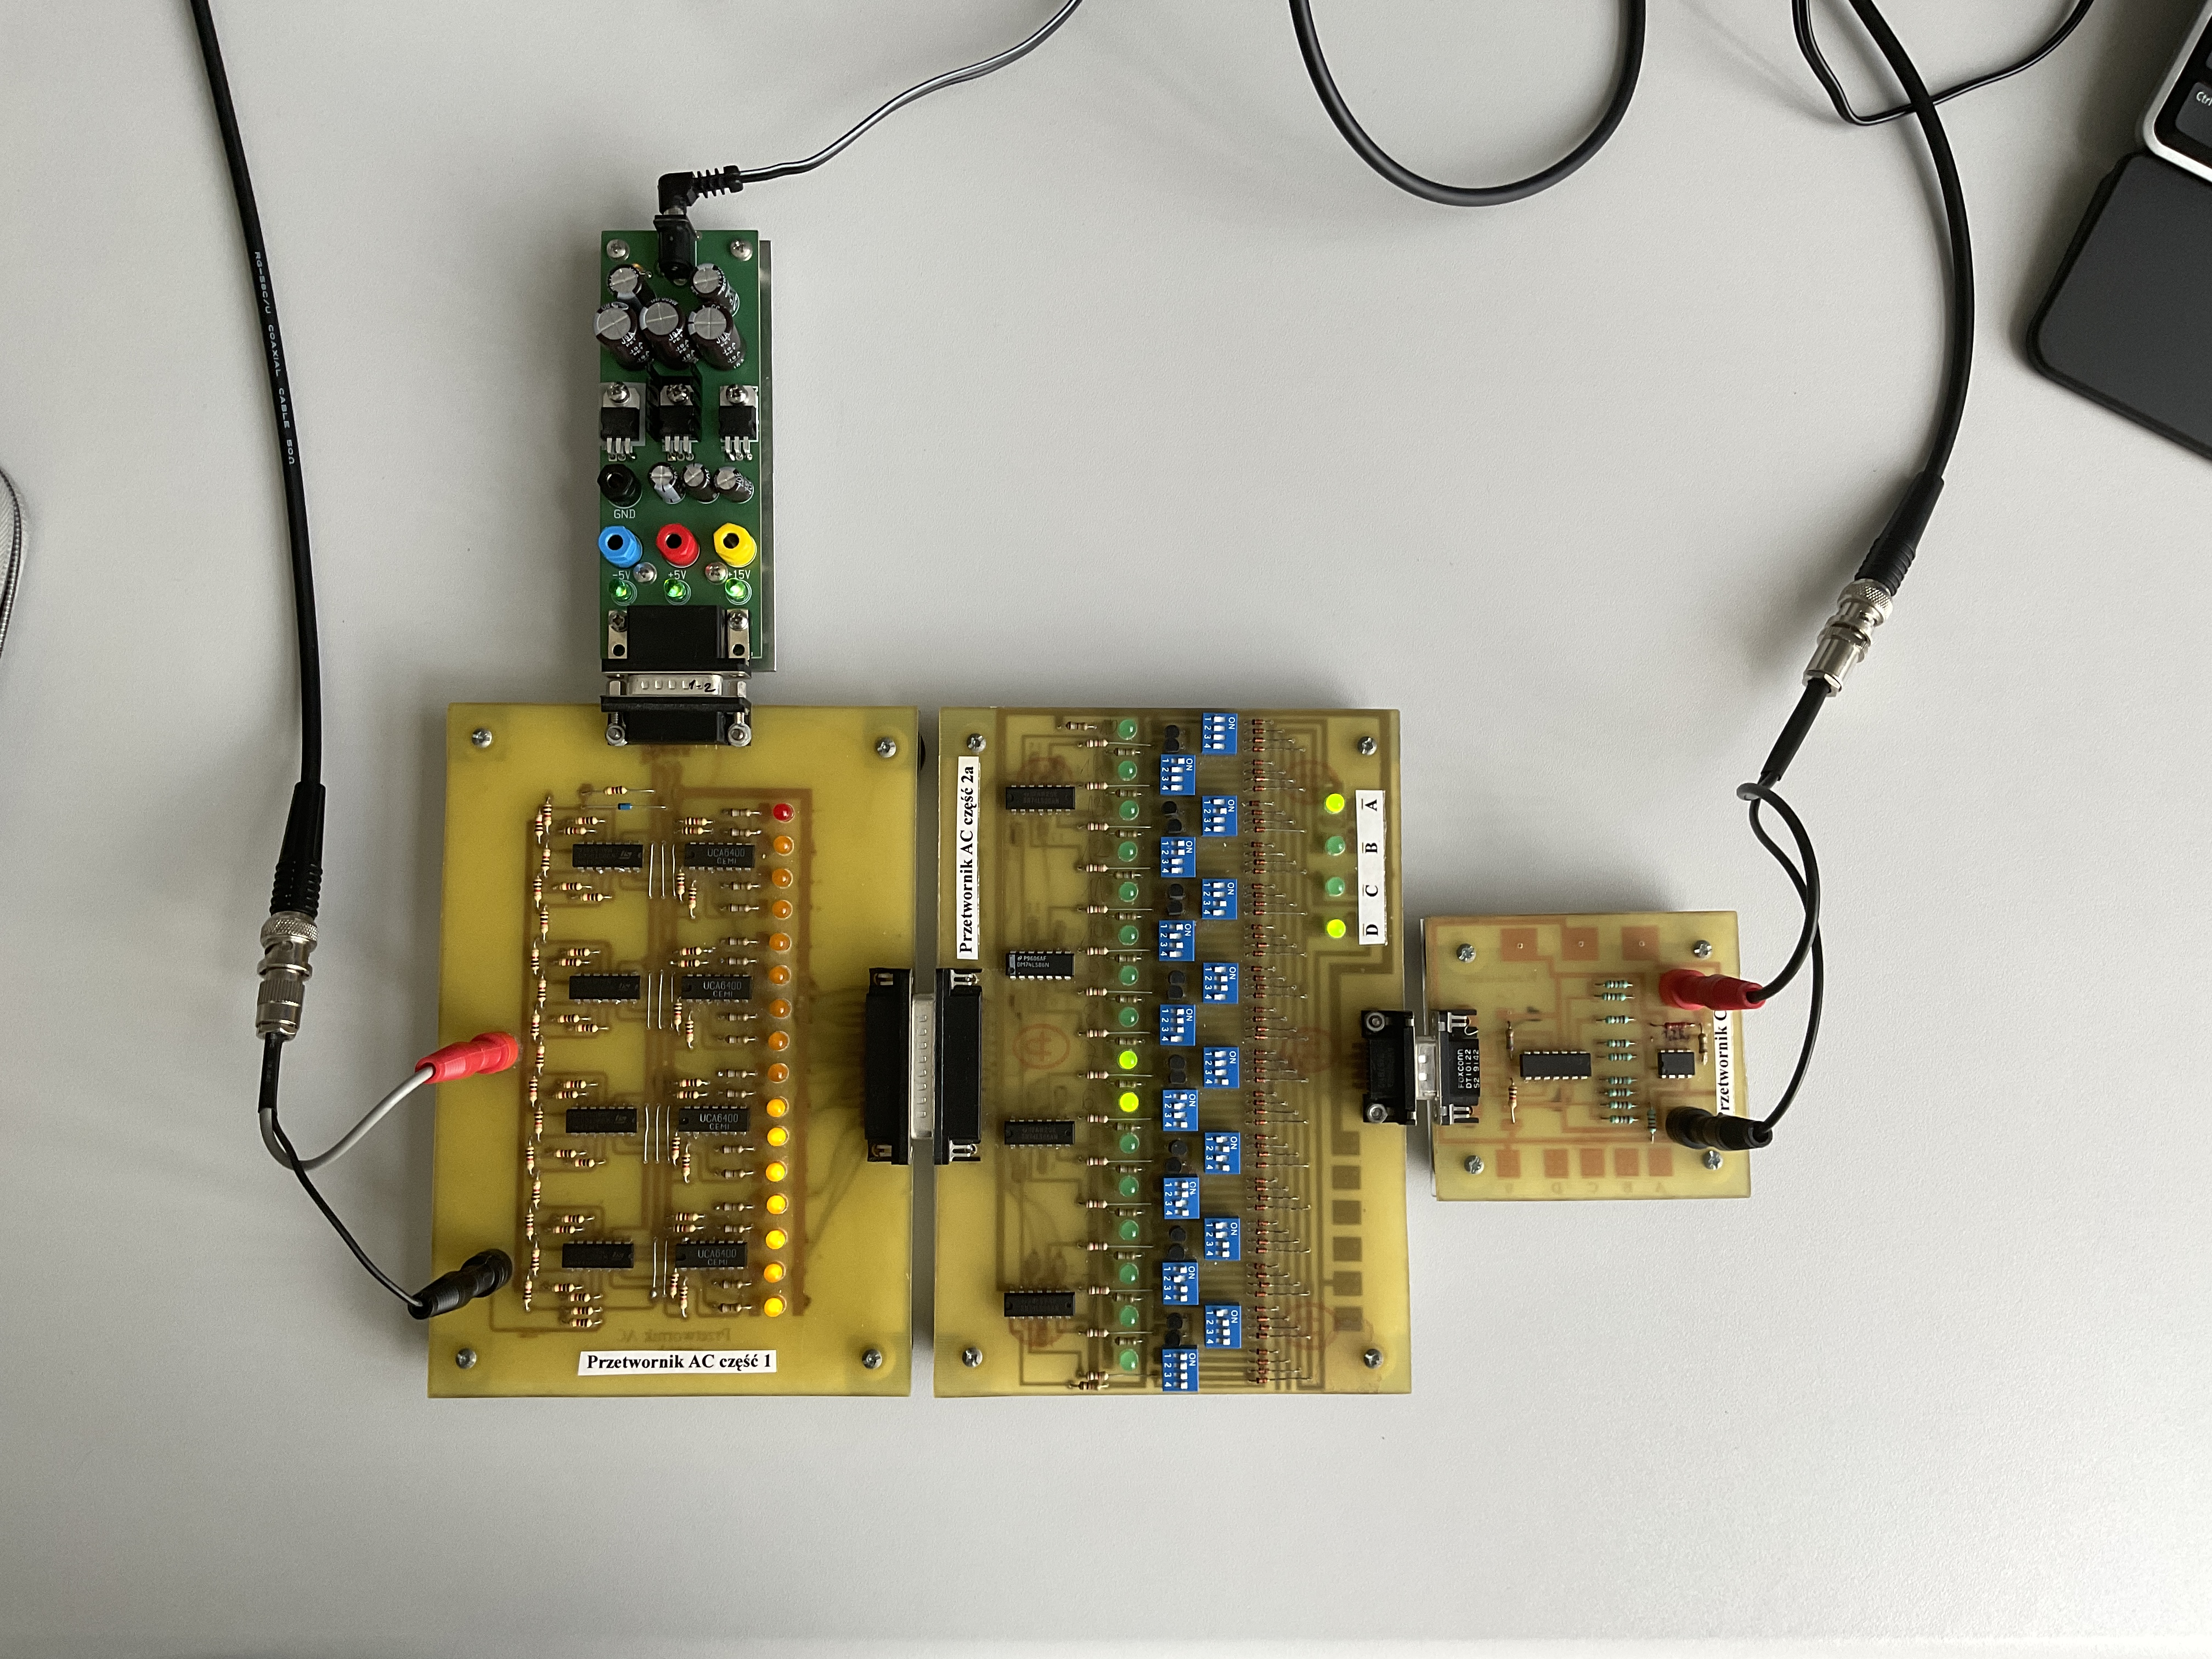
\includegraphics[width=8cm]{C1}
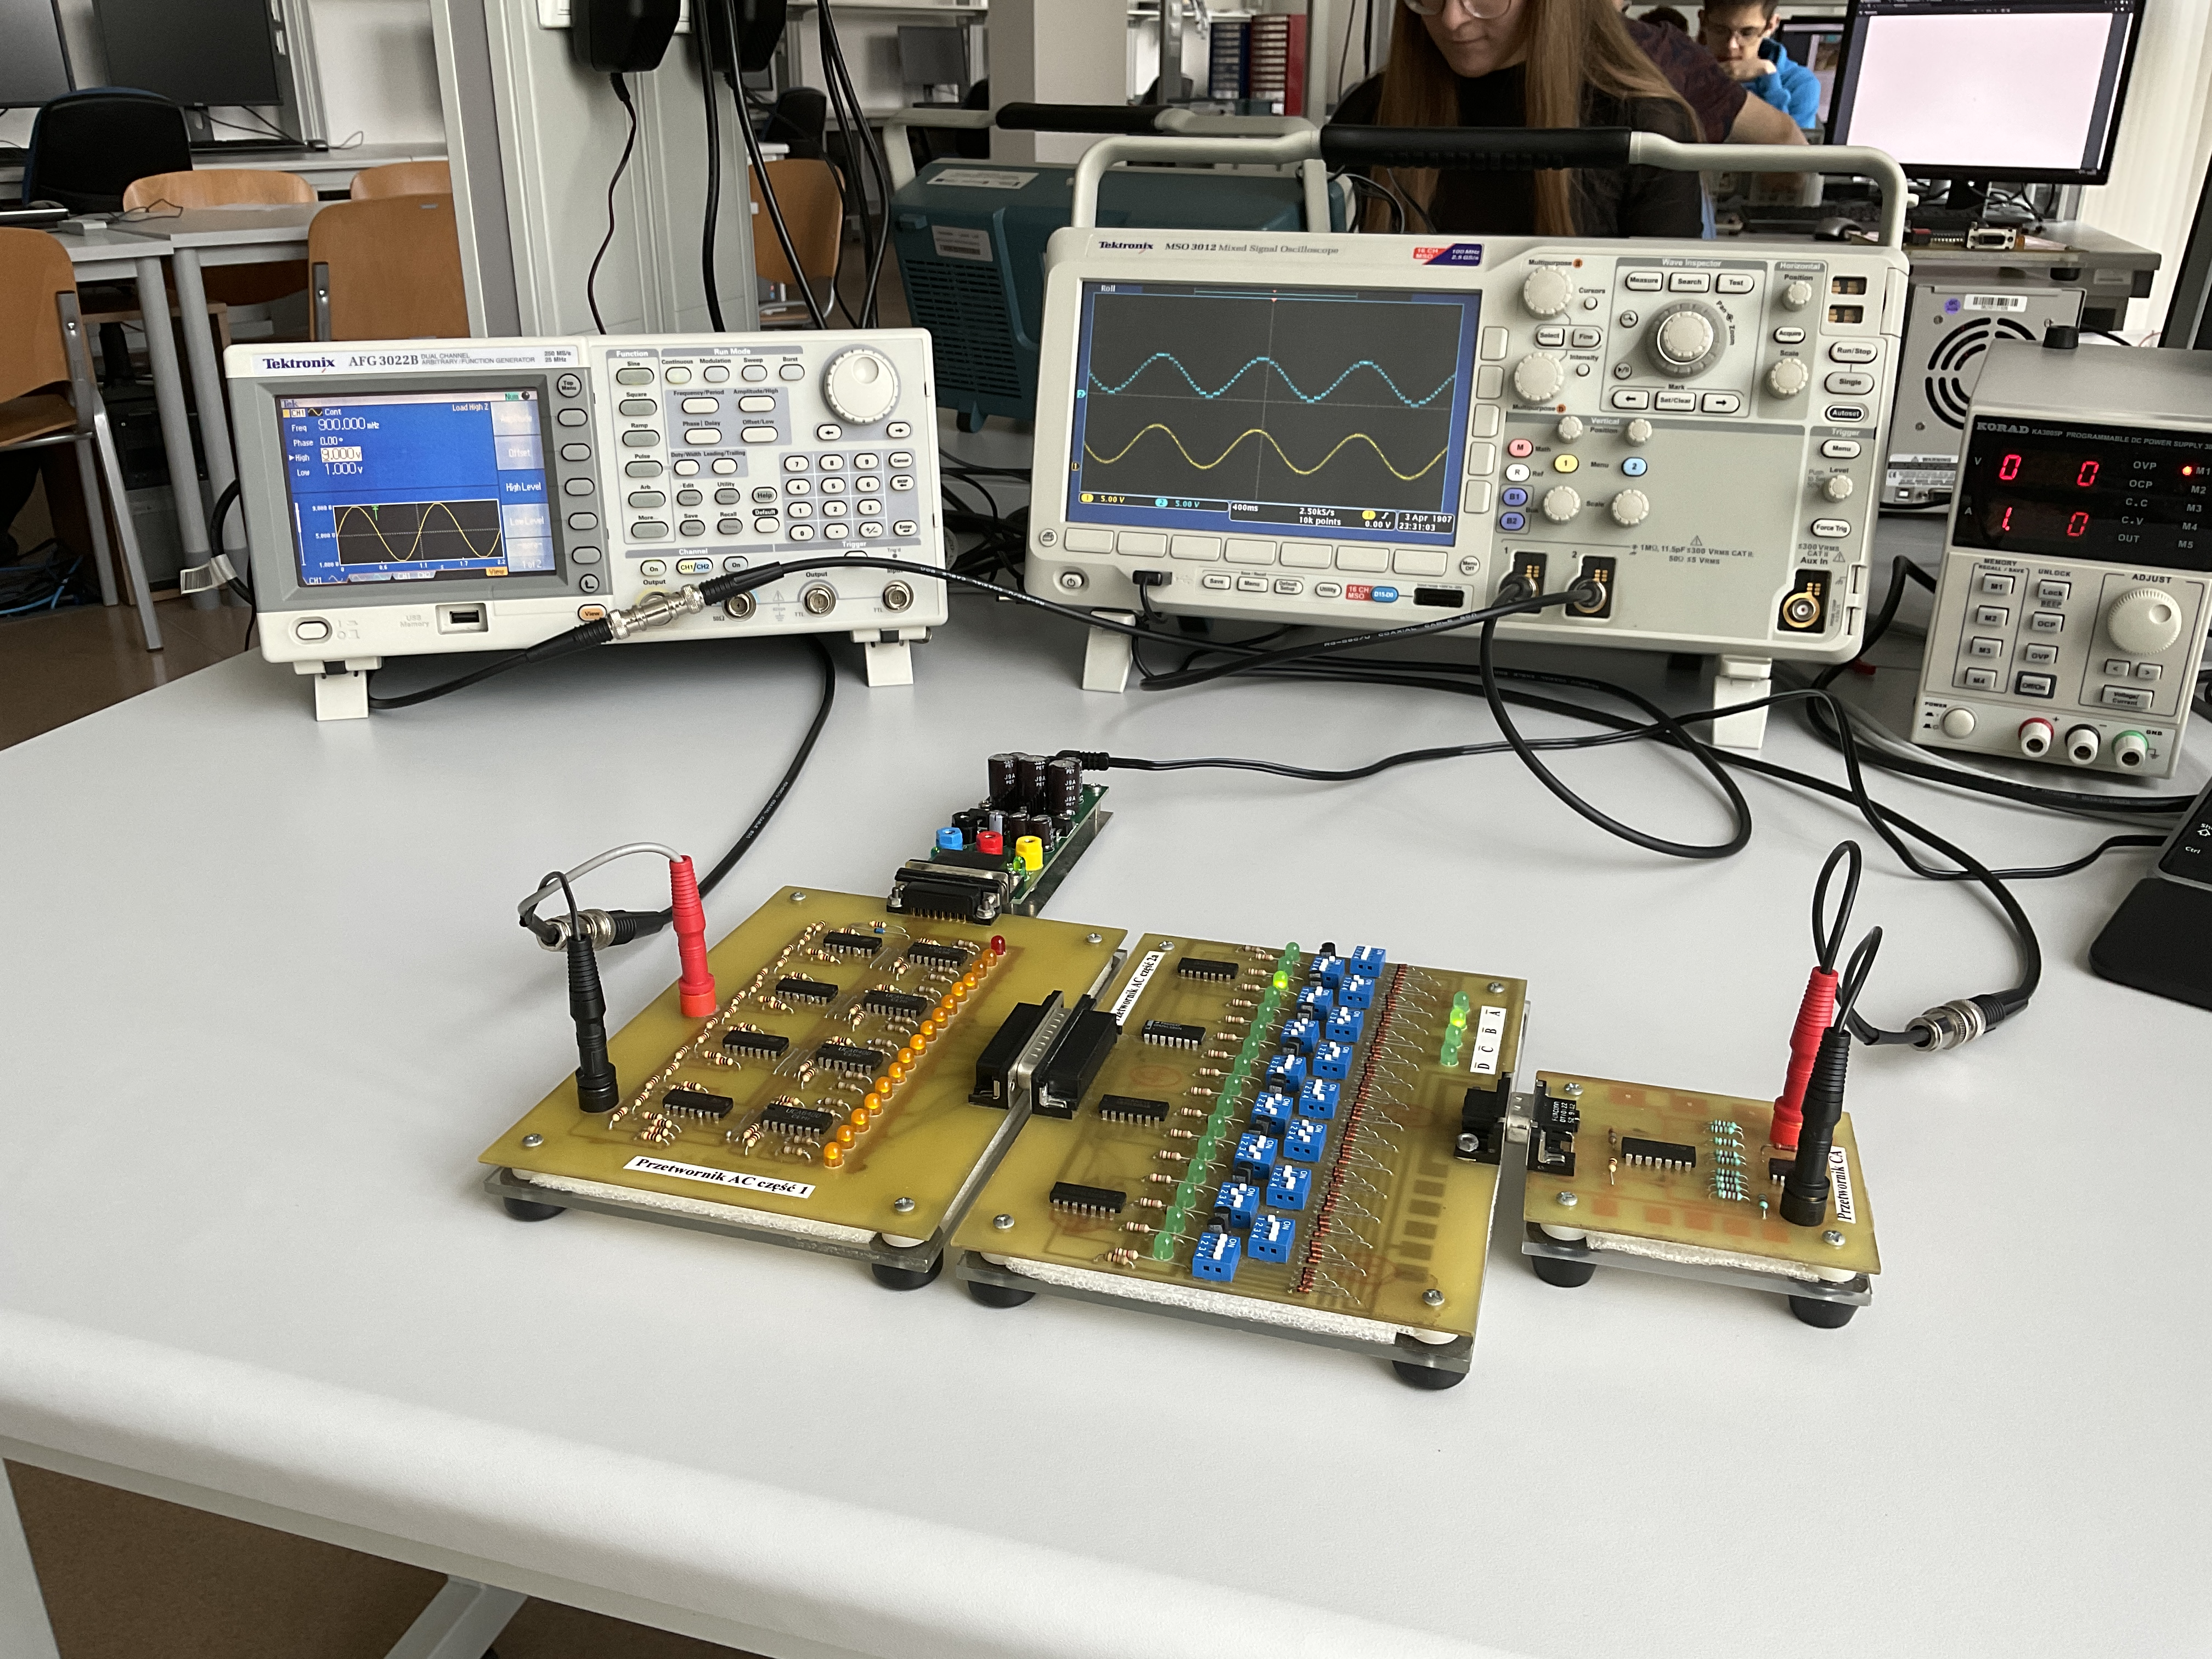
\includegraphics[width=8cm]{C2}
\centering
\captionsetup{labelformat=empty}
\caption{Zdjęcie 3: Przetwornik A/C zmontowany przy użyciu transkodera RPP-S. \\ Zdjęcie 4: przetwornik podłączony do oscyloskopu i generatora.}
\end{figure}

Zmontowałem przetwornik jak na zdjęciu 3. Przy pomocy \textit{switchy} na bloku transkodera zaprogramowałem układ tak, by na wyjściu cyfrowym pojawiały się liczby od 0 do 15 zapisane w naturalnym kodzie binarnym. Na wejście układu podałem z generatora sygnał o częstotliwości $900 \ mHz$ i amplitudzie pomiędzy $1 \ V$ a $9 \ V$. Zarówno wyjście generatora jak i wyjście układu przetwornika podłączyłem do oscyloskopu. Działanie całego układu prezentuję na filmiku znajdującym się w załączniku numer 1.

\newpage
\begin{figure}[H]
\includegraphics[width=16cm]{A0}
\centering
\captionsetup{labelformat=empty}
\caption{Wykres 1: Przebiegi sygnałów wyjściowych generatora (żółty) i przetwornika A/C (niebieski).}
\end{figure}

\newpage
Badając rozdzielczość napięciową konwertera podawałem na wejście układu napięcie stałe z zasilacza i zmieniałem je o $0.01 \ V$. Zapisywałem "wartości graniczne napięcia", czyli wartości napięcia, dla których załączył się kolejny komparator (zaświeciła się kolejna dioda na module komparatorów). Zmierzone przeze mnie wartości wyniosły:

\begin{center}
\begin{tabular}{| c | c |}
\hline
\textbf{Dioda} & \textbf{Napięcie} \\
\hline
1 & $0.35 \ V$ \\
\hline
2 & $1.04 \ V$ \\
\hline
3 & $1.73 \ V$ \\
\hline
4 & $2.43 \ V$ \\
\hline
5 & $3.12 \ V$ \\
\hline
6 & $3.81 \ V$ \\
\hline
7 & $4.5 \ V$ \\
\hline
8 & $5.19 \ V$ \\
\hline
9 & $5.88 \ V$ \\
\hline
10 & $6.57 \ V$ \\
\hline
11 & $7.26 \ V$ \\
\hline
12 & $7.95 \ V$ \\
\hline
13 & $8.64 \ V$ \\
\hline
14 & $9.34 \ V$ \\
\hline
15 & $10.03 \ V$ \\
\hline
16 (przester) & $10.37 \ V$ \\
\hline
\end{tabular}
\end{center}

Zmontowany przeze mnie przetwornik A/C jest przetwornikiem czterobitowym (binarna liczba stanowiąca jego wyjście ma 4 bity. Zatem liczba poziomów reprezentacji tego przetwornika wynosi $2^4 = 16$. Dzieląc teoretyczny zakres $0 - 10 \ V$ w którym działa przetwornik na liczbę jego poziomów reprezentacji, zakładając że są one równe otrzymamy teoretyczną rozdzielczość napięciową: $r_V = \frac{10 \ V}{16} = 0.625 \ V$. \\

Zmierzona przeze mnie rozdzielczość napięciowa jest średnią różnic pomiędzy dwoma kolejnymi "wartościami granicznymi napięcia", podanymi w tabeli powyżej.
Jest więc równa:

$$ r_V = \frac{(1.04 - 0.35) + (1.73 - 1.04) + \ldots + (10.03 - 9.36)}{14} \approx 0.692 \ V $$

\newpage
\textbf{3.4} Użycie modułu z pamięcią SRAM. Zmodyfikowanie powyższej konfiguracji zastępując transkoder RPP-S transkoderem z pamięcią SRAM. Postępując analogicznie jak opisano w punktach 3.2 i 3.3 zaprogramowanie pamięć SRAM i sprawdzenie działanie przetwornika. Zaprojektowanie układu w ten sposób aby amplituda sygnału po konwersji ulegała odwróceniu. \\

\begin{figure}[H]
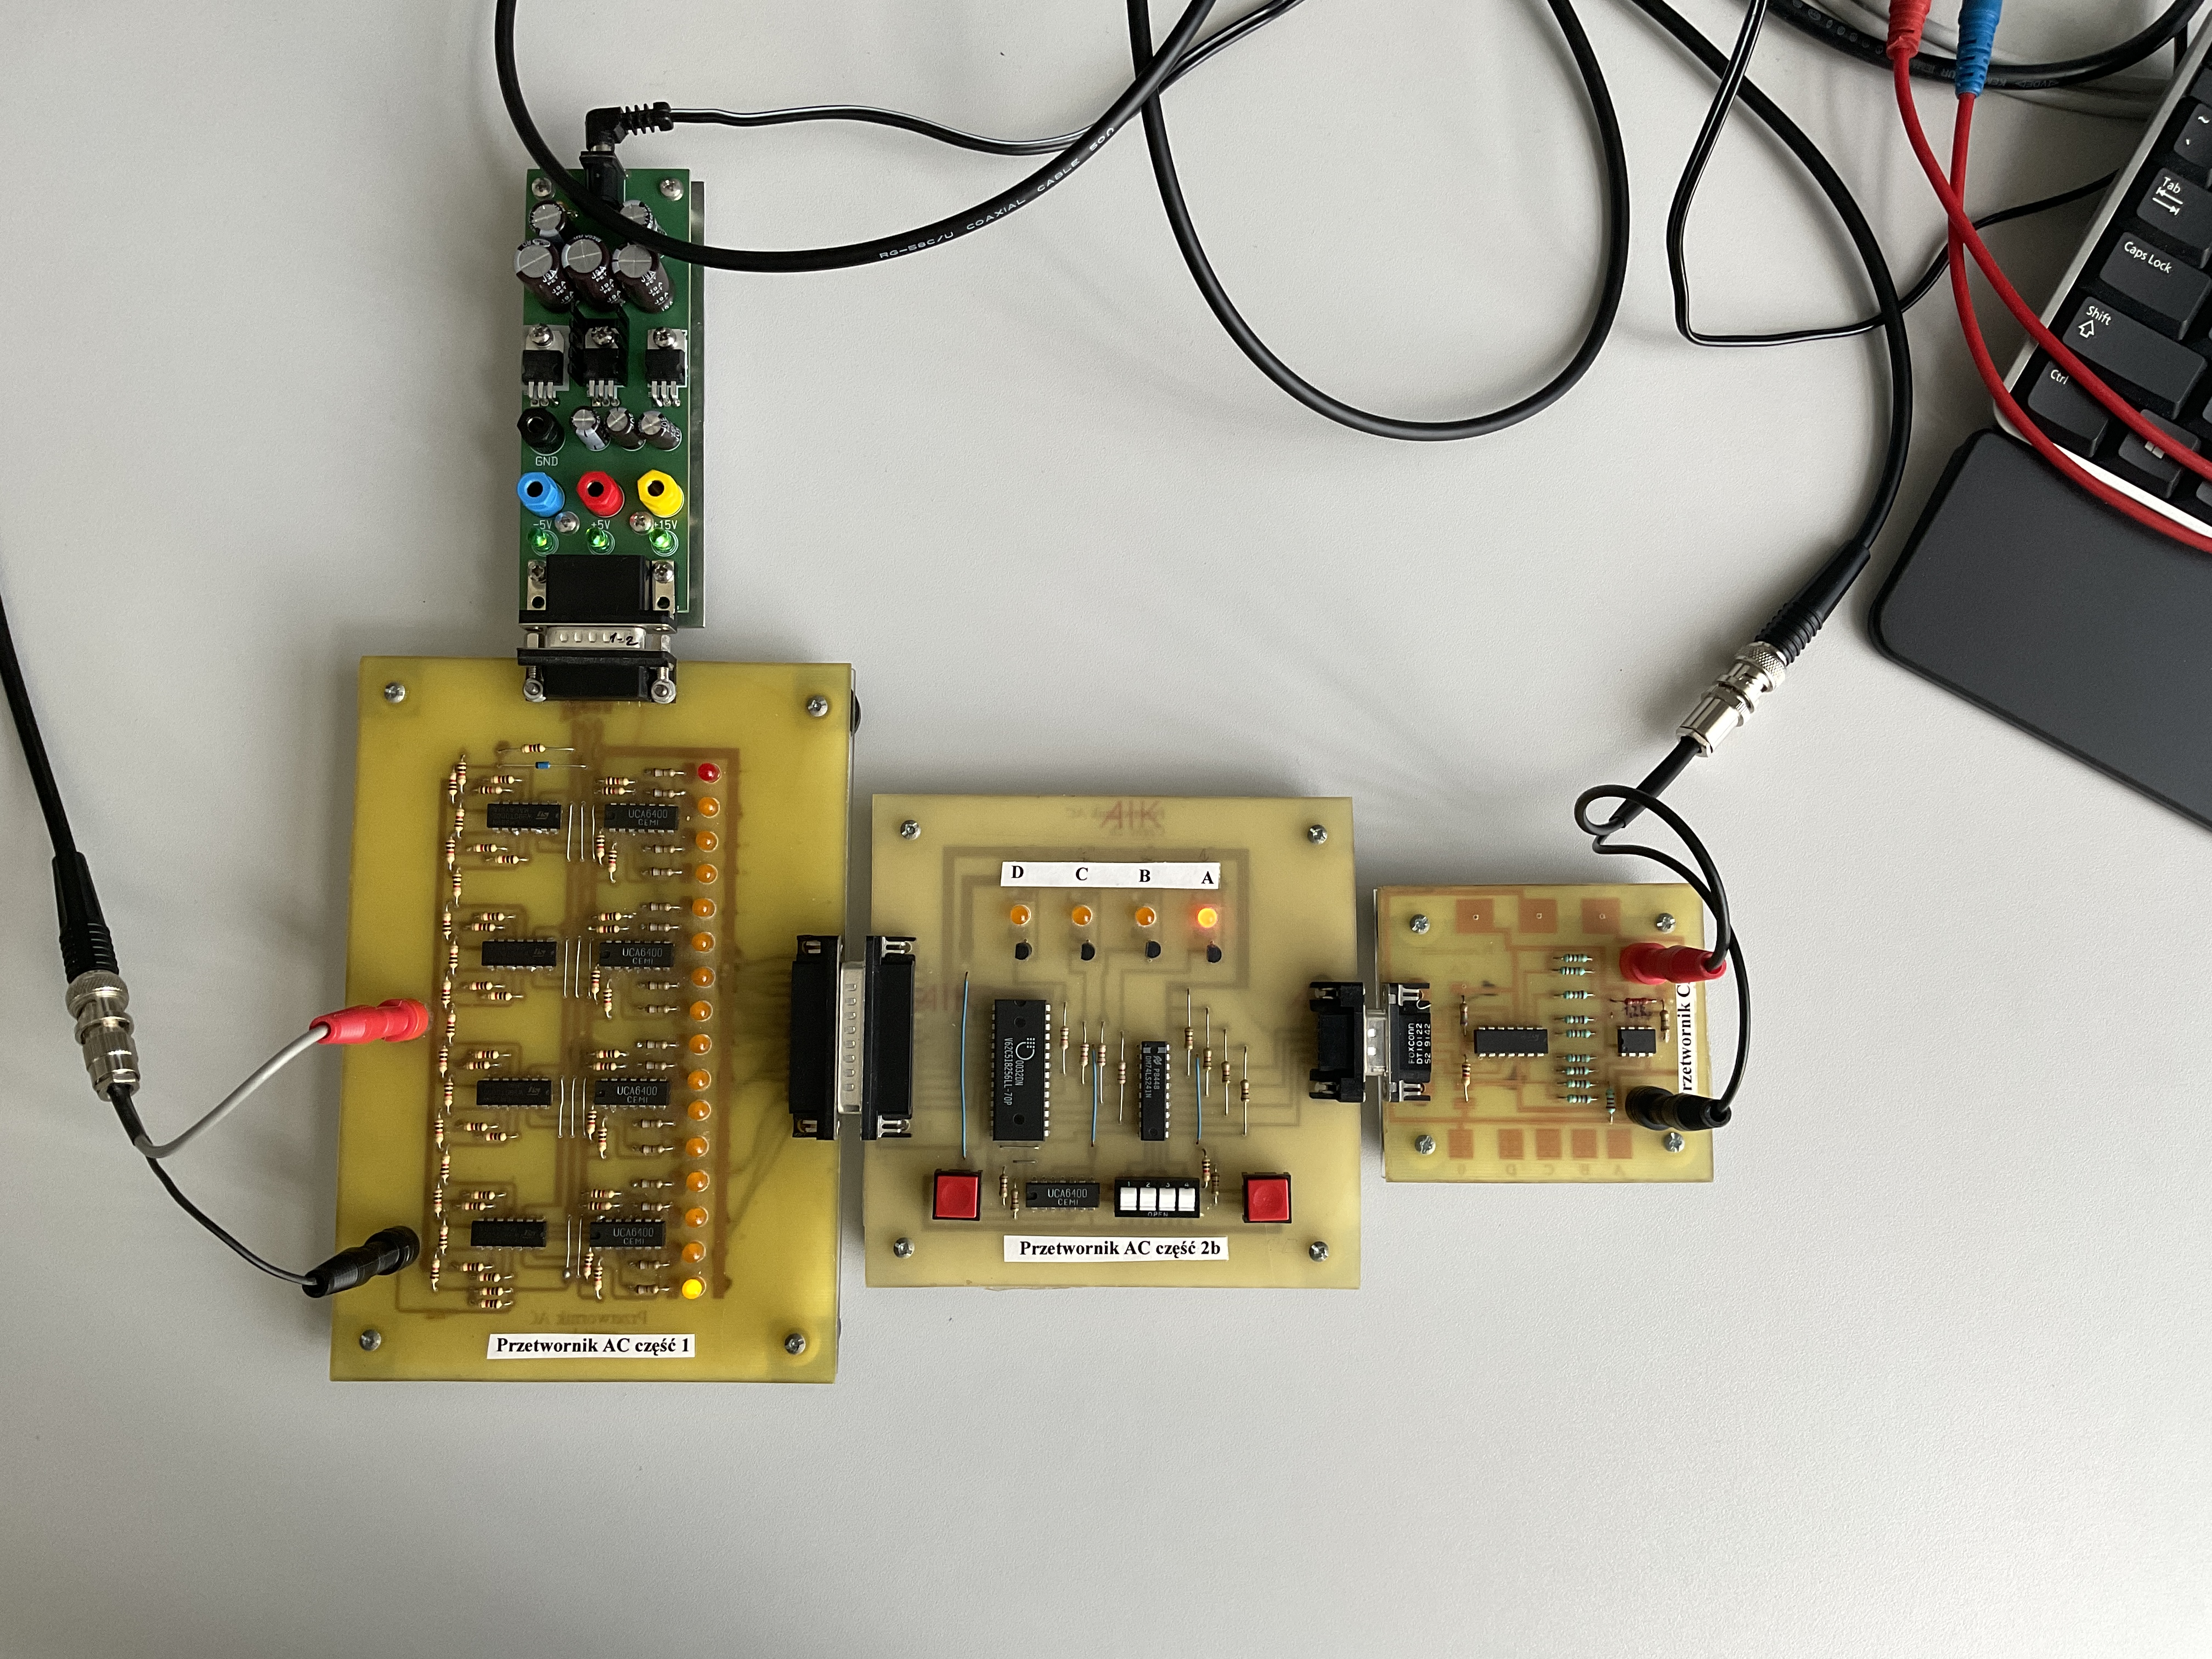
\includegraphics[width=8cm]{C4}
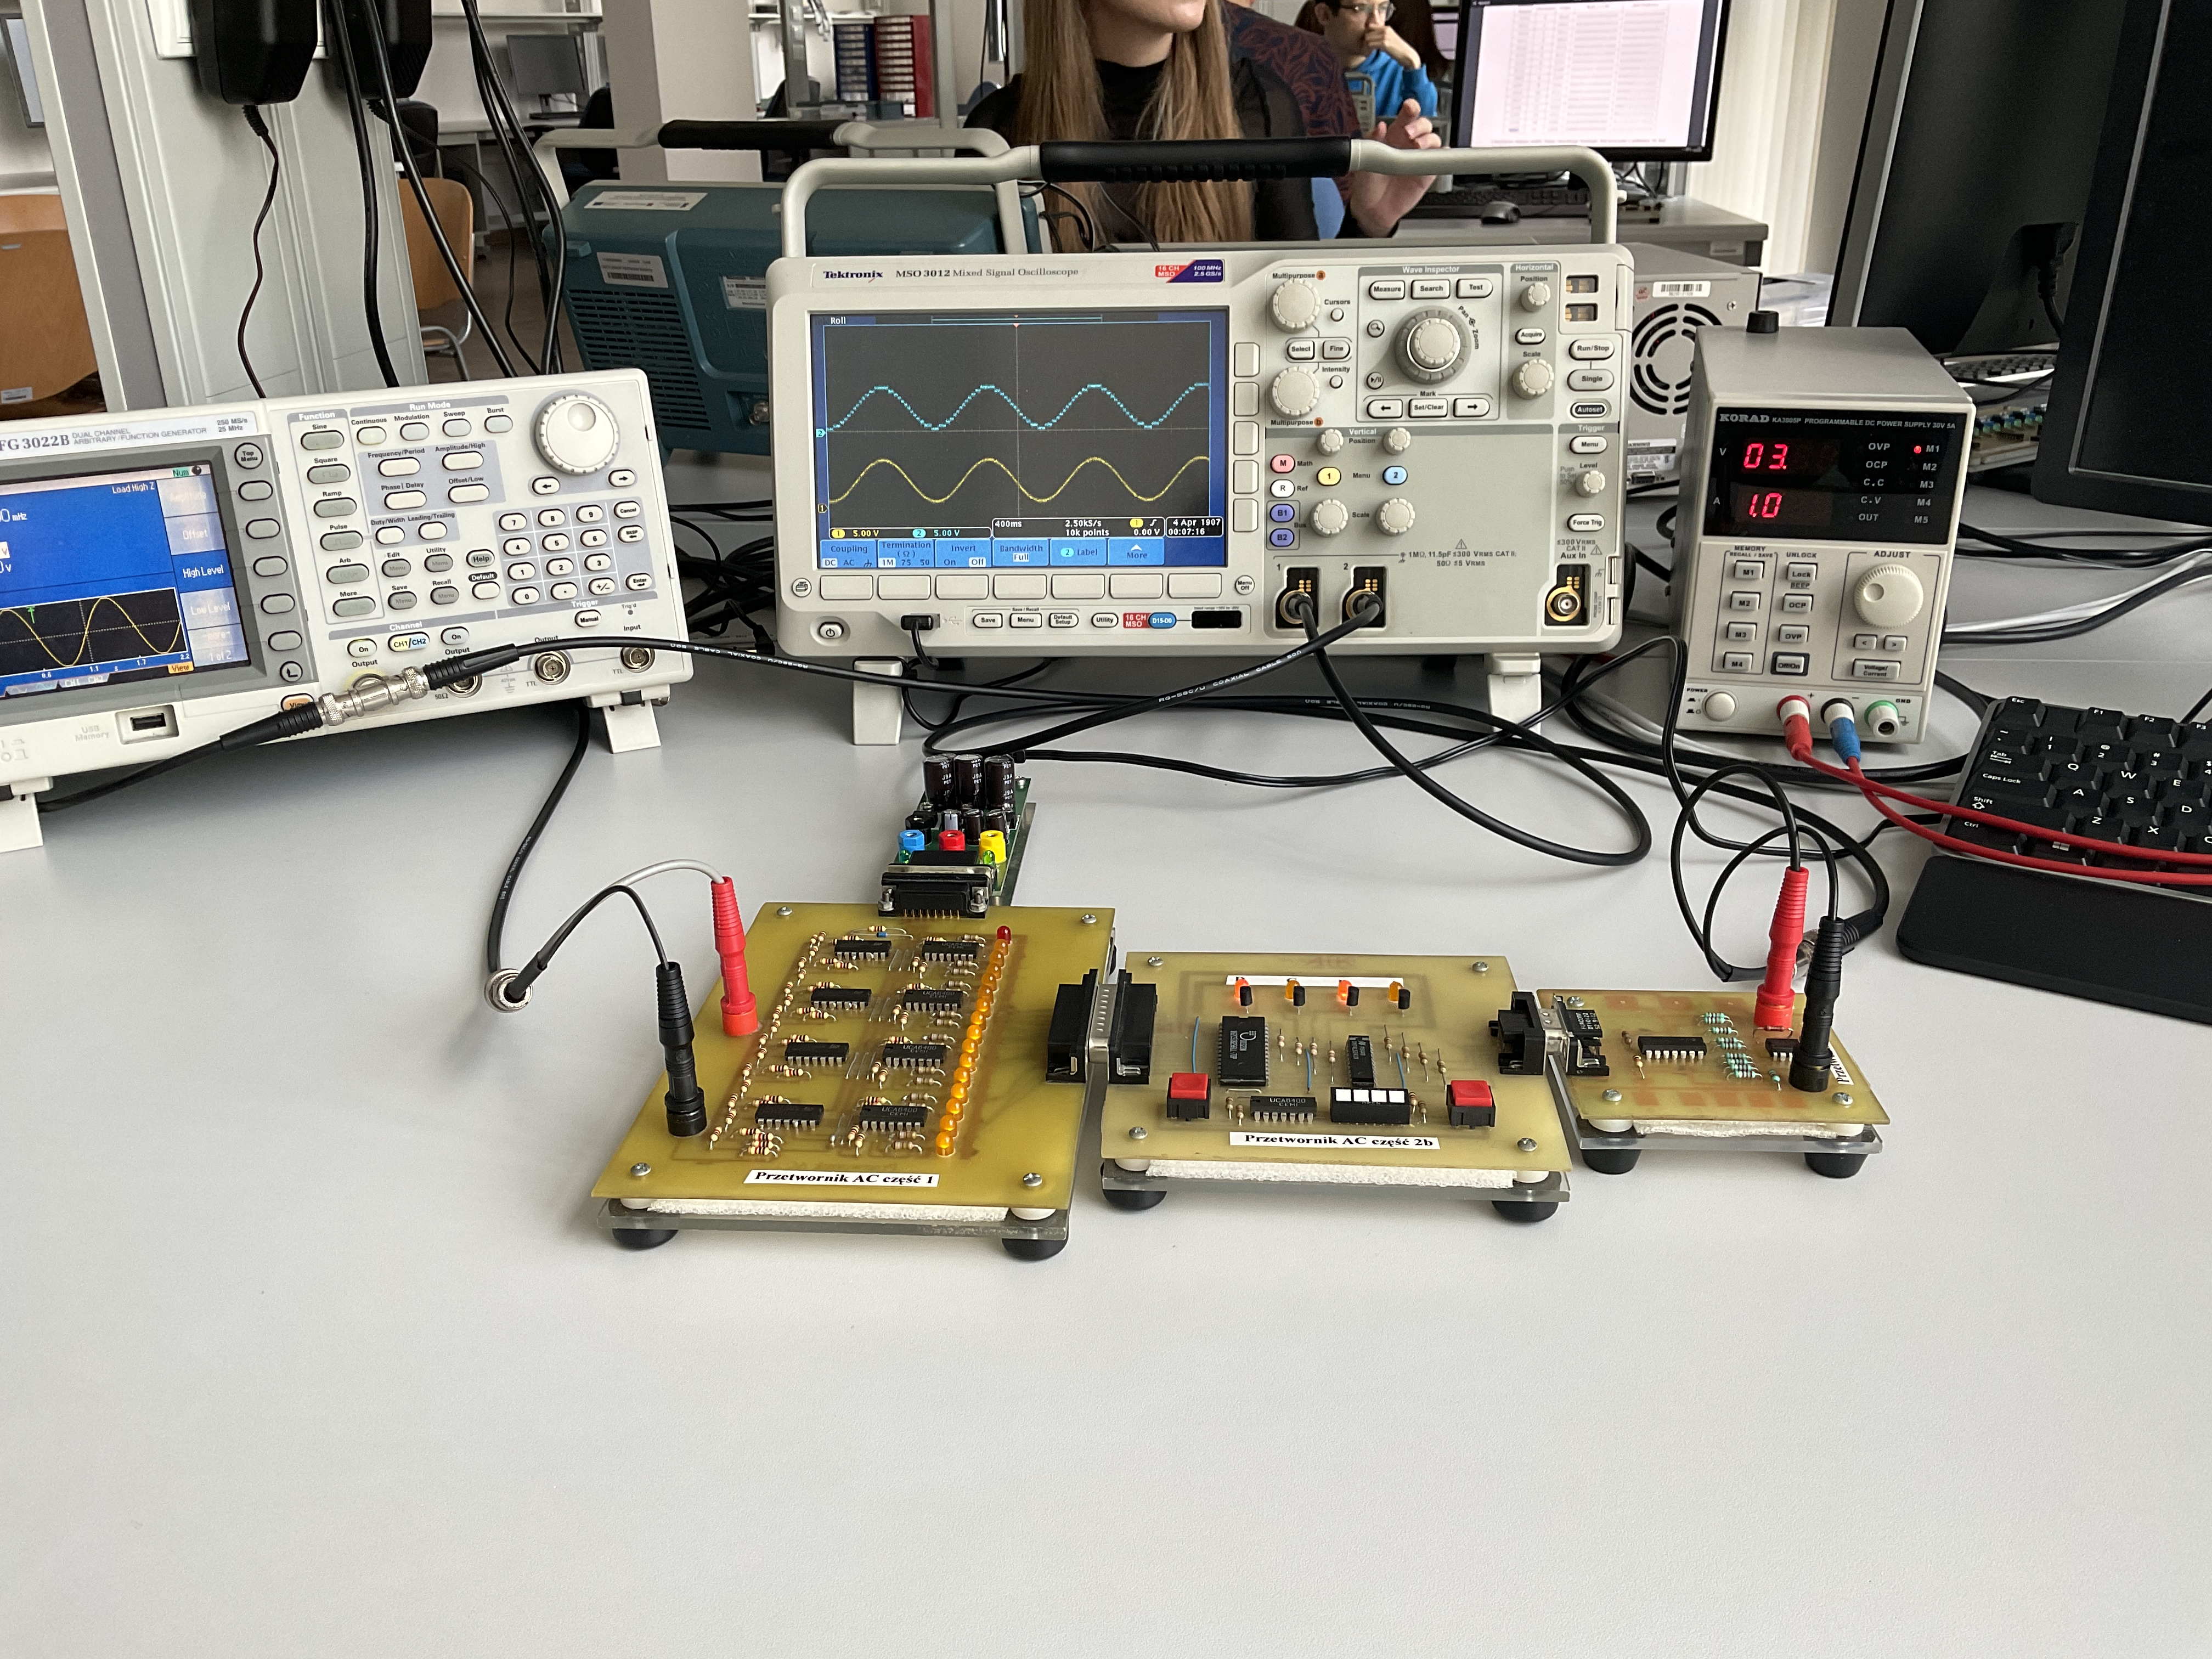
\includegraphics[width=8cm]{C5}
\centering
\captionsetup{labelformat=empty}
\caption{Zdjęcie 5: Przetwornik A/C zmontowany przy użyciu transkodera z pamięcią SRAM. \\ Zdjęcie 6: przetwornik podłączony do oscyloskopu i generatora.}
\end{figure}

Wymieniając w poprzedniej konfiguracji środkowy blok zmontowałem przetwornik A/C korzystający z transkodera z pamięcią RAM. Na początku podawałem na wejście układu prąd stały o określonych wartościach, tak aby na linie adresowe transkodera podawać kolejne adresy. Przy pomocy \textit{switchy} i przycisków na bloku transkodera zaprogramowałem układ tak, by na wyjściu cyfrowym pojawiały się liczby od 0 do 15 zapisane w naturalnym kodzie binarnym. \\

Następnie na wejście układu podałem z generatora sygnał o częstotliwości $900 \ mHz$ i amplitudzie pomiędzy $1 \ V$ a $9 \ V$. Zarówno wyjście generatora jak i wyjście układu przetwornika podłączyłem do oscyloskopu. Działanie całego układu prezentuję na filmiku znajdującym się w załączniku numer 1.

\newpage
Następnie, zmieniając wejście spowrotem na napięcie stałe przeprogramowałem transkoder tak, aby w swojej pamięci zawierał liczby od 15 do 0, czyli w odwrotnej kolejności. Po przeprogramowaniu podpiąłem na wejście generator (taka sama fala jak wcześniej) i obserwowałem przebiegi wejścia i wyjścia.

\begin{figure}[H]
\includegraphics[width=16cm]{A2}
\centering
\captionsetup{labelformat=empty}
\caption{Wykres 2: Przebiegi sygnałów wyjściowych generatora (żółty) i przetwornika A/C (niebieski).}
\end{figure}

Na wykresie można zobaczyć odwróconą amplitudę sygnału po konwersji - jest to wynik tego, że w komórkach adresowych znajdują się liczby binarne od 15 do 0, a nie, jak wcześniej od 0 do 15. W przypadku punktów 3.2 i 3.3 wartości były ustalone przełącznikami na stałe w kolejności rosnącej, dlatego amplituda nie ulegała odwróceniu.

\newpage
\textbf{3.5} Dla przebiegu sinusoidalnego określenie zakresu częstotliwości, w której przetwornik działa poprawnie. \\

Prawidłowe działanie przetwornika jest ograniczone przez czas propagacji sygnałów przez komparatory, które muszą zdążać się załączać i wyłączać podczas przetwarzania sygnału. Jeżeli sygnał zmieni wartość zanim komparator osiągnie docelowy stan to sygnał wyjściowy zostanie zdegenerowany. Można wyciągnąć stąd też wniosek, że częstotliwość nie jest niczym ograniczana od dołu — znaczy to, że może być dowolnie niska. \\

Aby odkryć częstotliwość graniczną górną podawałem na wejście przetwornika falę sinusoidalną z generatora o wartościach oscylujących pomiędzy $0$ a $8 \ V$ i stopniowo zwiększałem częstotliwość.

\begin{figure}[H]
\includegraphics[width=8cm]{A7}
\includegraphics[width=8cm]{A6}
\centering
\captionsetup{labelformat=empty}
\caption{Wykres 3: $20 \ kHz$ \ Wykres 4: $40 \ kHz$}
\end{figure}

\begin{figure}[H]
\includegraphics[width=8cm]{A5}
\includegraphics[width=8cm]{A4}
\centering
\captionsetup{labelformat=empty}
\caption{Wykres 5: $70 \ kHz$ \ Wykres 6: $110 \ kHz$}
\end{figure}

\begin{figure}[H]
\includegraphics[width=8cm]{A3}
\centering
\captionsetup{labelformat=empty}
\caption{Wykres 7: $340 \ kHz$}
\end{figure}

Analizując przebiegi wyjścia przetwornika zauważyłem, że fale poniżej $20 \ kHz$ nie są zniekształcone i na pewno mogłyby być odczytane przez urządzenie cyfrowe. Przy $40 \ kHz$ na wyjściu widoczne jest to, że zmiana jednej wartości na drugą nie jest natychmiastowa i ta część "schodków", która powinna być pionowa zostaje pochylona. Powyżej tej częstotliwości sygnał staje się już za bardzo zdegenerowany i niemożliwy do odczytania przez inny układ cyforwy. Widać to dokładnie na wykresie numer 5, przy fali o częstotliwości $70 \ kHz$. Powyżej tej granicy sygnał wyjściowy staje się zupełnie zdegenerowany: na wykresie 6 przypomina właściwie falę sinusoidalną a na wykresie 7 ma stłumioną amplitudę i kształt trójkątny. \\

Wobec powyższych obserwacji możemy powiedzieć, że przetwornik może działać prawidłowo w zakresie od $0 \ Hz$ do około $40 \ kHz$.

\newpage
\paragraph{Zadanie 4. \\}

\textbf{4.1} Zapoznanie się ze schematem przetwornika A/C działającego w oparciu o przetwornik C/A i jego elementami: przetwornikiem C/A, komparatorem, generatorem sygnału zegarowego, licznikiem, rejestrem SAR i wyjściem na wyświetlacz.

\begin{figure}[H]
\includegraphics[width=16cm]{D3}
\centering
\captionsetup{labelformat=empty}
\caption{Schemat 4: Schemat blokowy przetwornika.}
\end{figure}

\begin{figure}[H]
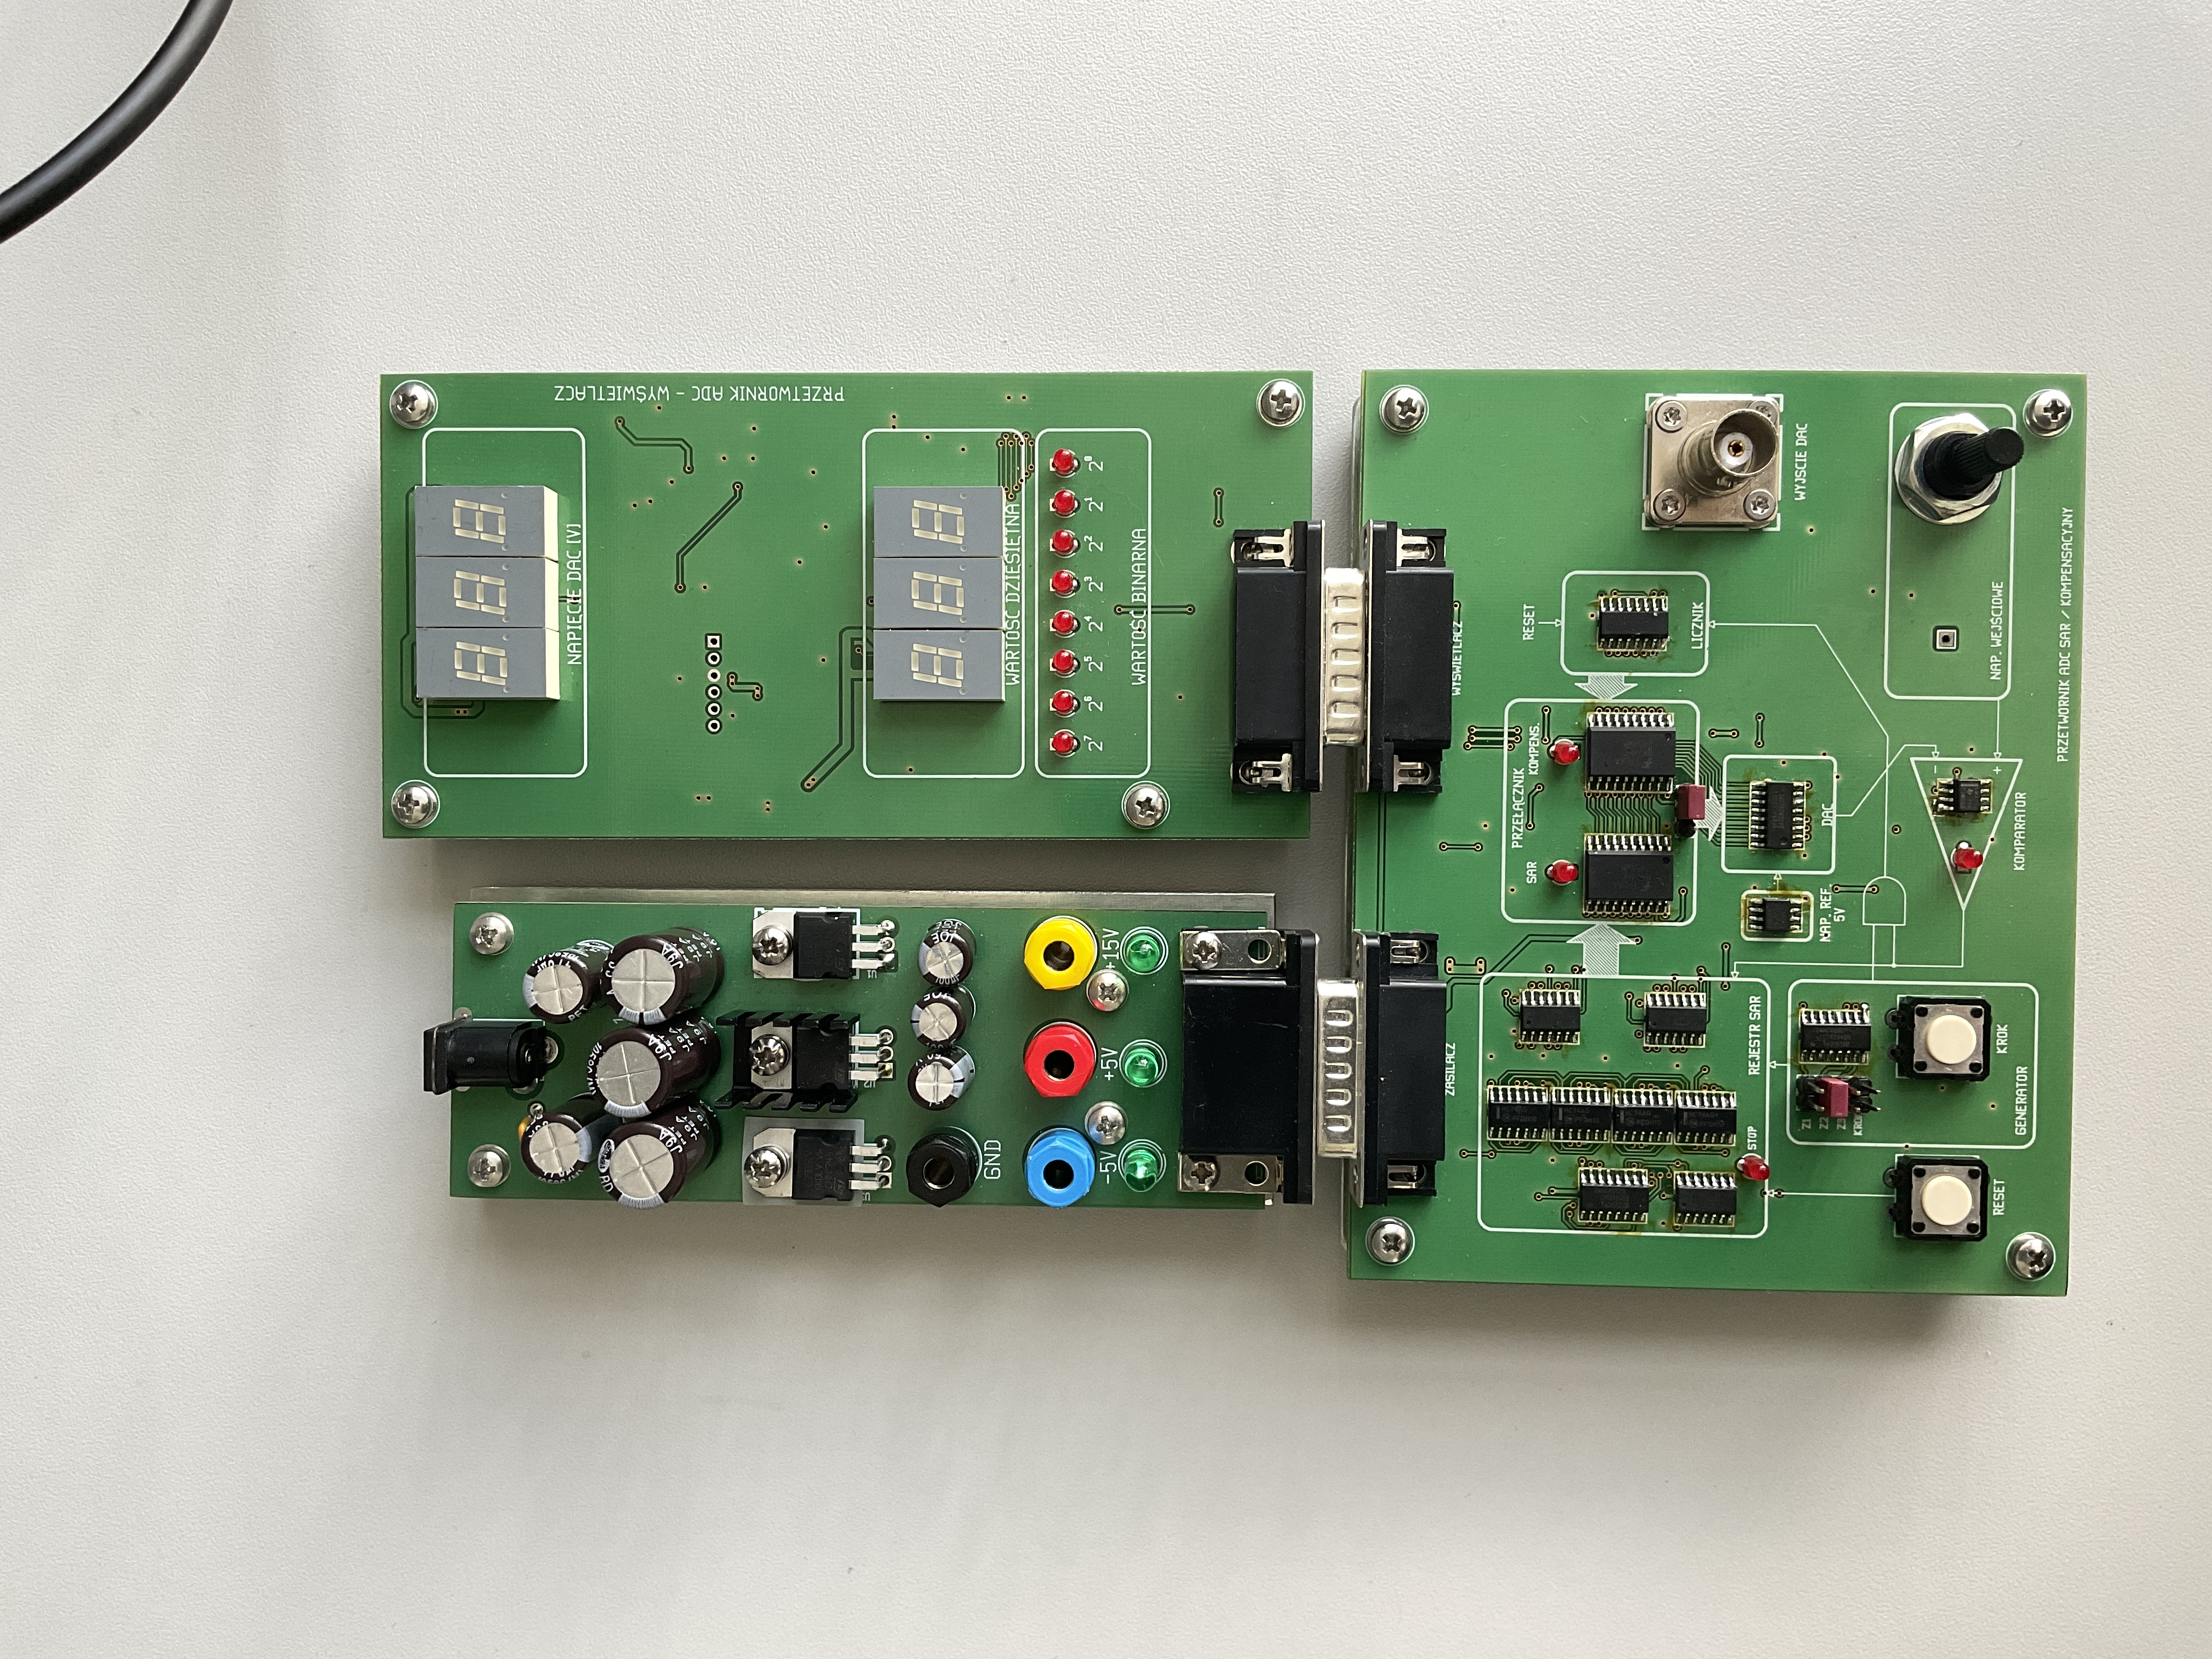
\includegraphics[width=15cm]{C6}
\centering
\captionsetup{labelformat=empty}
\caption{Zdjęcie 7: Połączony układ przetwornika A/C SAR.}
\end{figure}

\newpage
\textbf{4.2} Zbadanie poprawności działania przetwornika. \\

Przy pomocy potencjometru ustawiłem napięcie wejściowe na poziomie $3.0 \ V$. Zresetowałem licznik i wartość cyfrowa na wyświetlaczu wynosiła 153. Zmierzyłem napięcie na wyjściu przetwornika C/A oraz napięcie wejściowe (na potencjometrze) i potwierdziłem, że obydwie wartości wynoszą $3 \ V$. Filmik znajduje się w załączniku numer 2.\\

\textbf{4.3} Określenie rozdzielczości napięciowej przetwornika. \\

Jest to przetwornik ośmiobitowy ($2^8 = 256$) działający na zakresie od $0$ do $5 \ V$, więc jego teoretyczna rozdzielczość napięciowa wynosi $r_V = \frac{5 \ V}{256} = 0.01953125 \ V$. Obserwując zmianę napięcia pomiędzy dwoma sąsiednimi wartościami cyfrowymi zmierzyłem rozdzielczość $0.02 \ V$.

\begin{figure}[H]
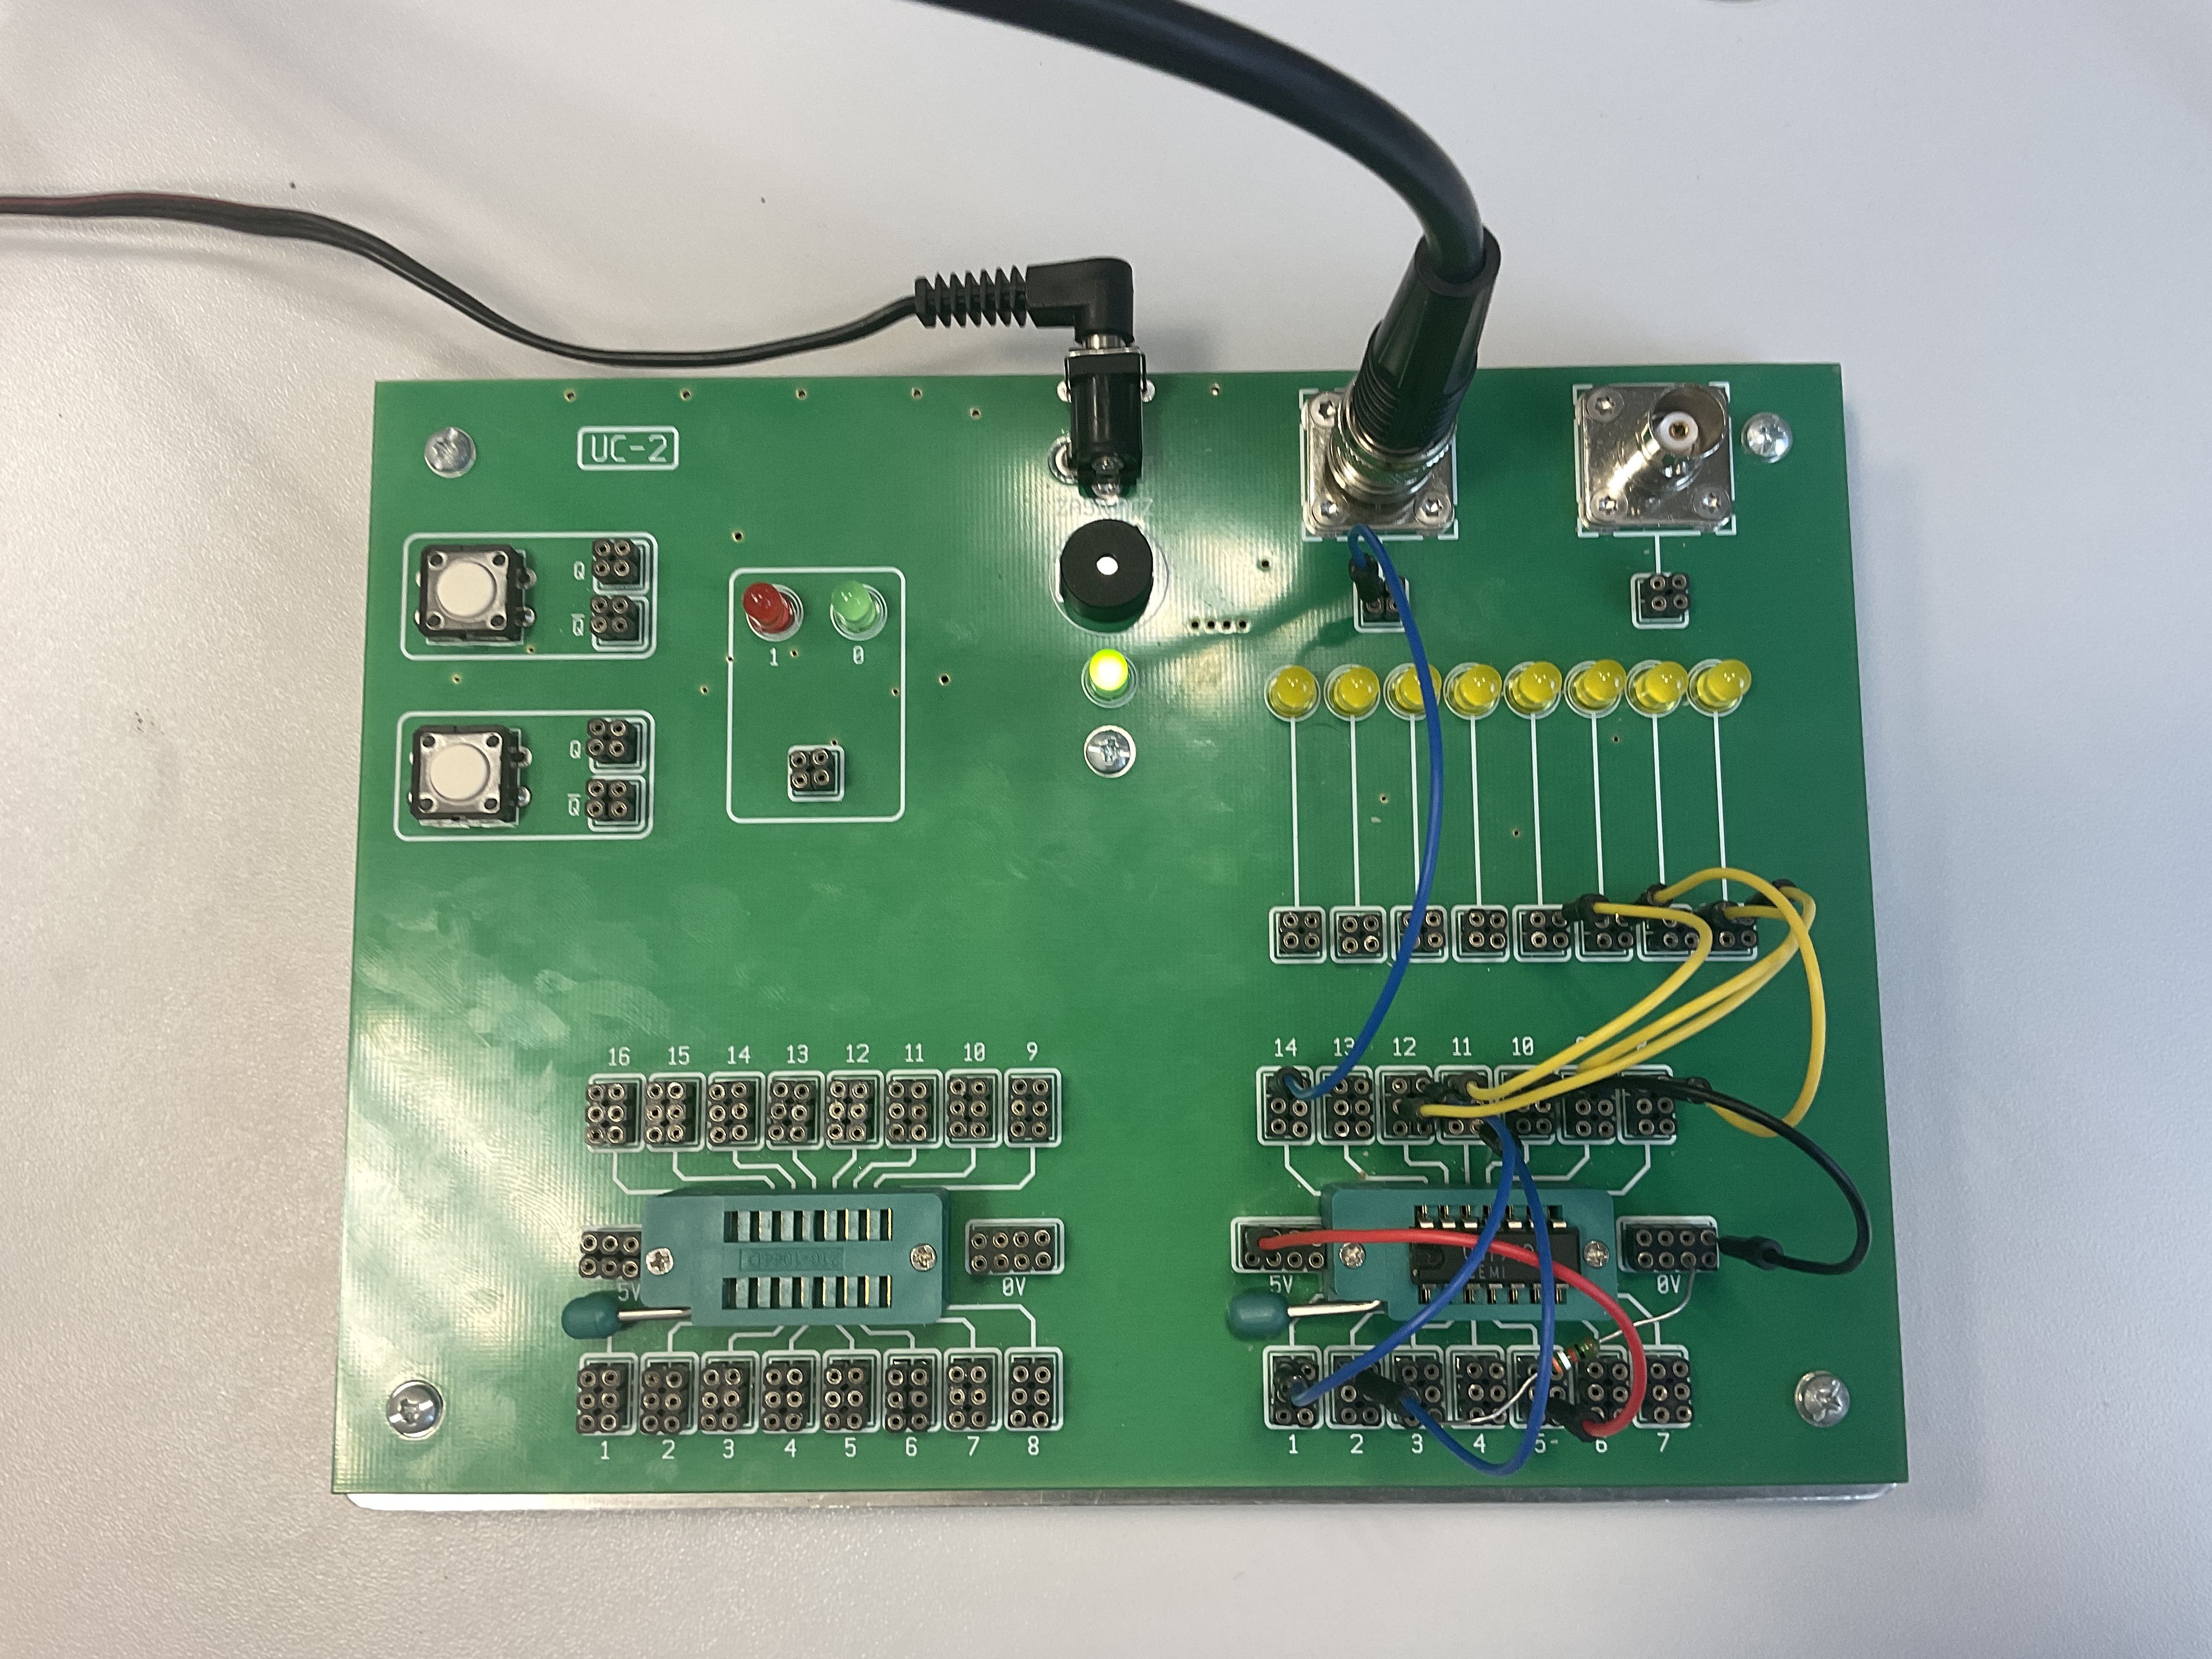
\includegraphics[angle=270, width=8cm]{C7}
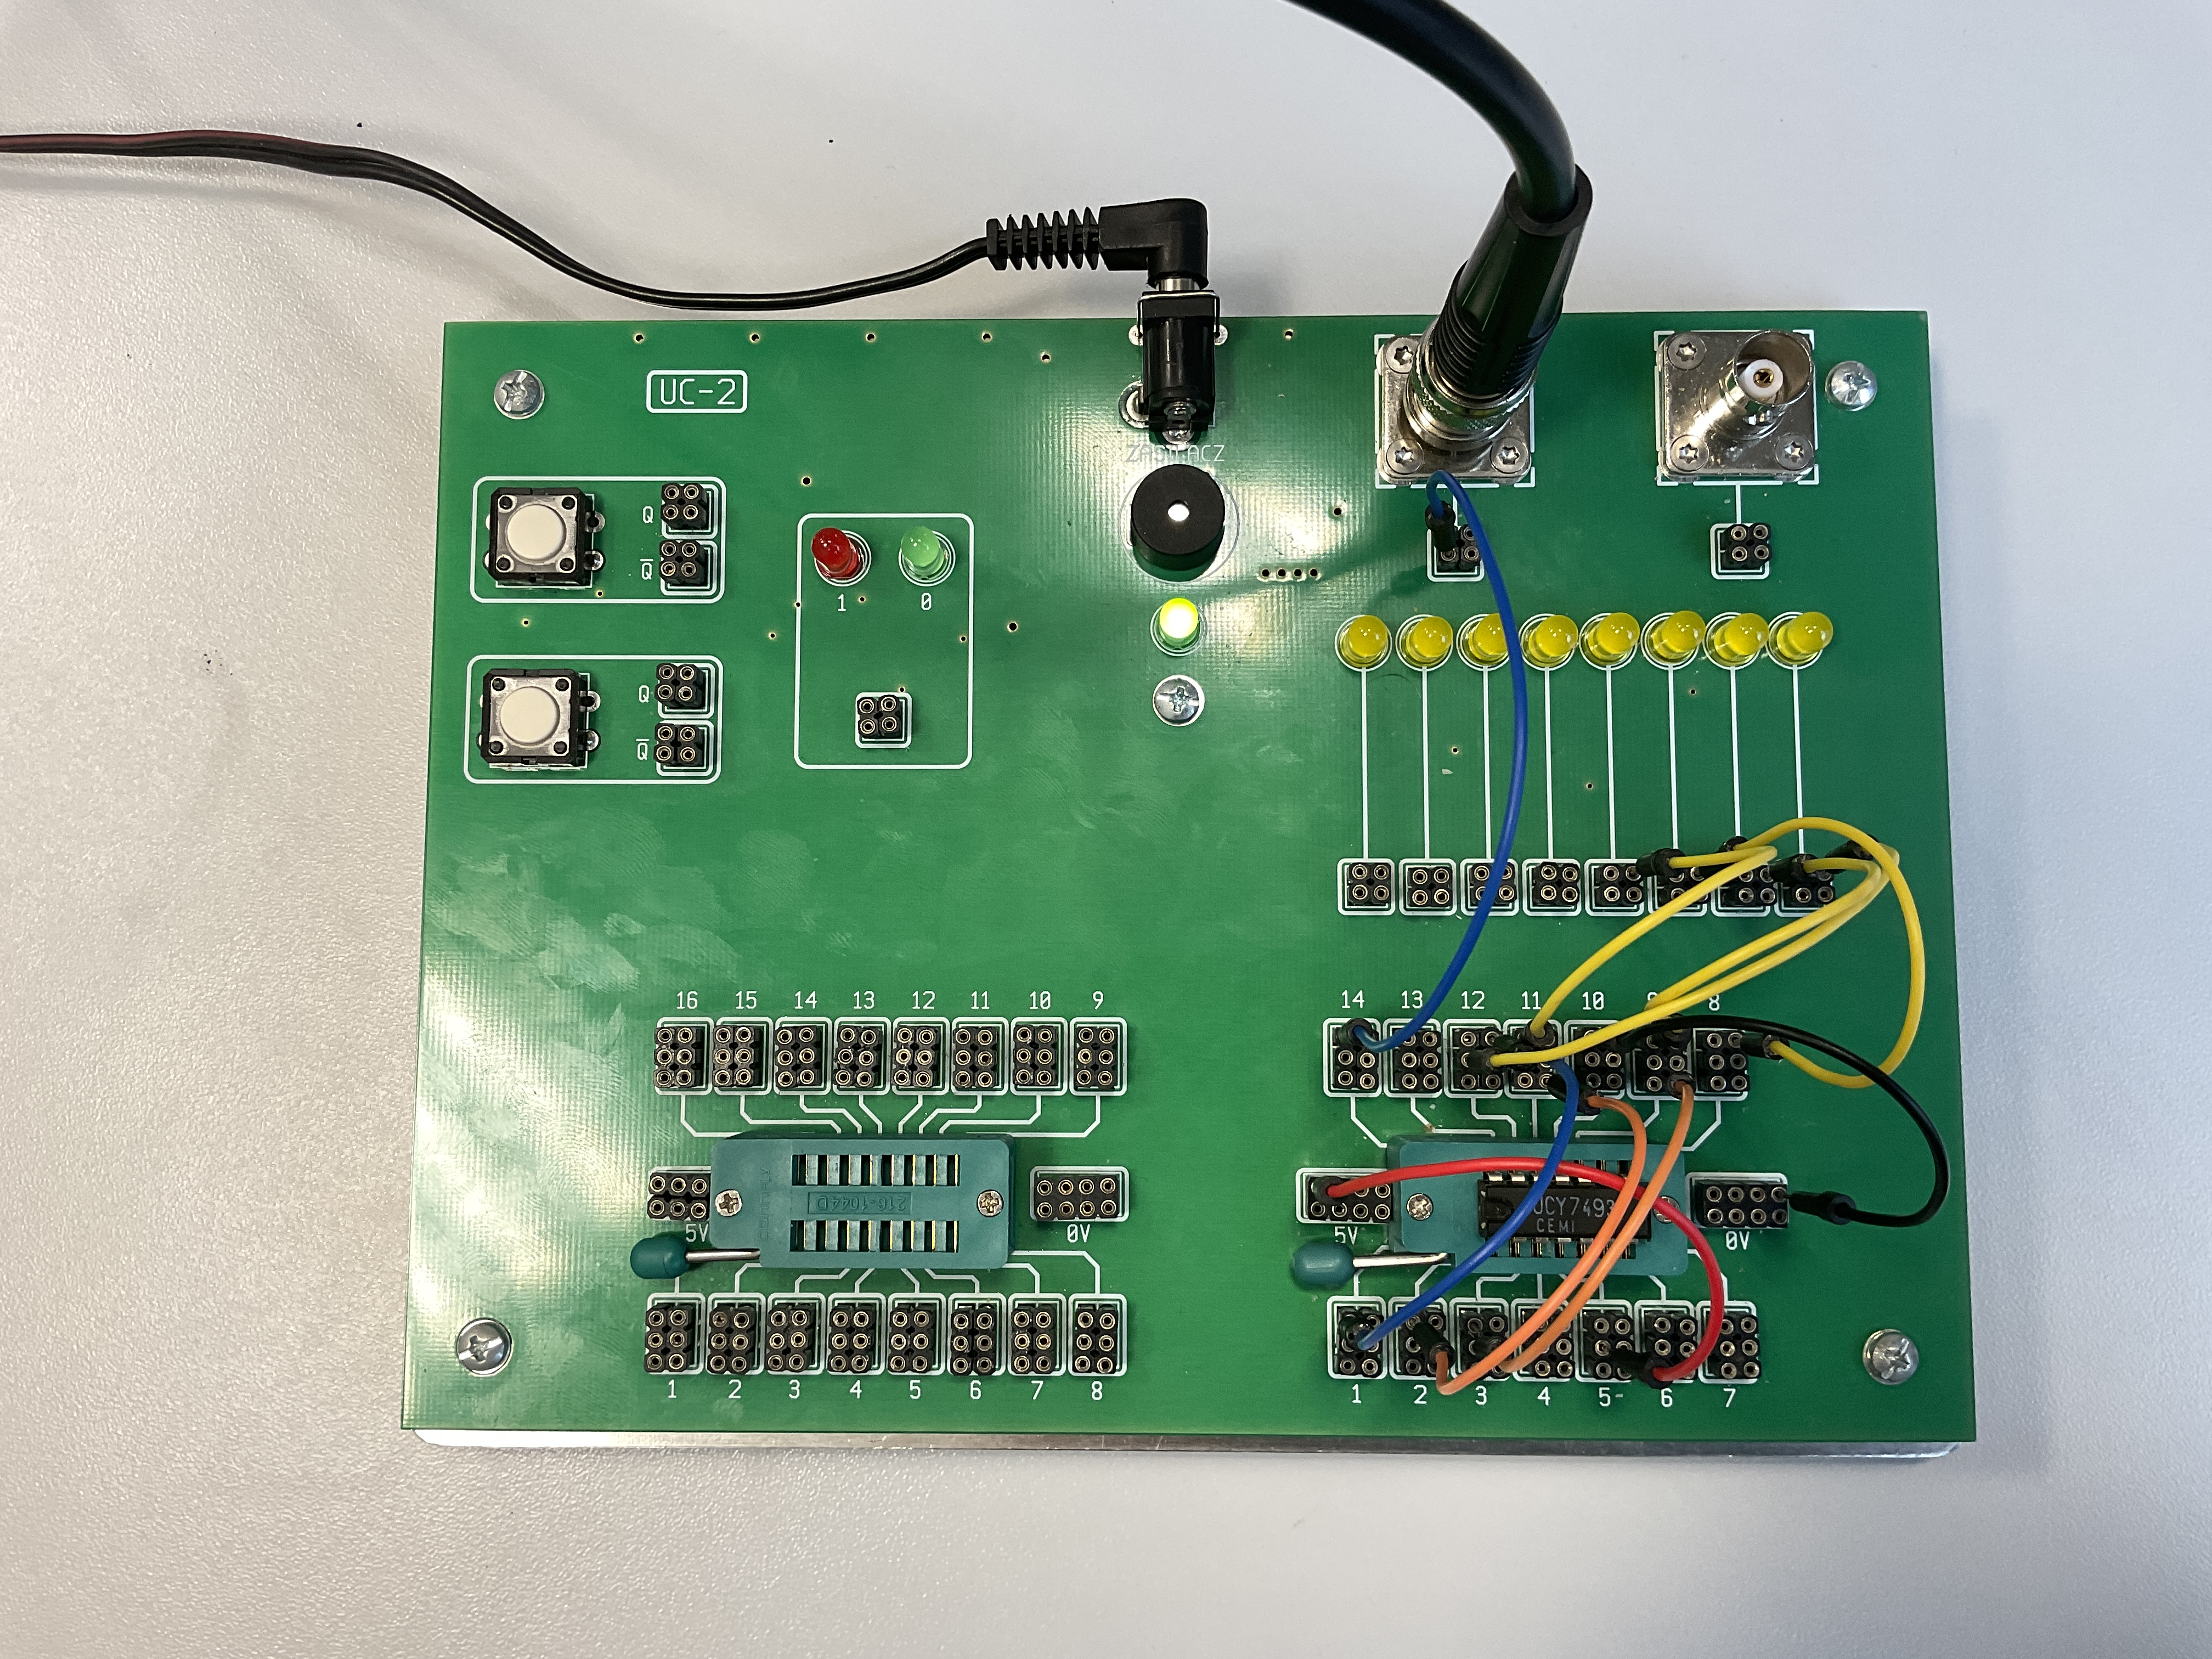
\includegraphics[angle=270, width=8cm]{C8}
\centering
\captionsetup{labelformat=empty}
\caption{Zdjęcia 8 i 9: Różnica napięcia pomiędzy wartością 010 a 011.}
\end{figure}

\newpage
\textbf{4.4} Określenie maksymalnej i minimalnej częstotliwości pracy przetwornika.

Ustawiłem napięcie wejściowe za pomocą potencjometru na wartość $5 \ V$. Zworkę regulacji częstotliwości ustawiłem w pozycji Z2. Obserwując przebieg wyjścia przetwornika ustaliłem, że od momentu resetu zanim sygnał na wyjściu osiągnie wartość $5 \ V$ mija $29.32 \ s$. Zatem częstotliwość wynosi:

$$f_{Z2} = \frac{1}{\frac{29.32 \ s}{255}} = 8.6971350614 \ Hz $$

Powtórzyłem pomiar przy zworce ustawionej w pozycji Z3 - czas wyniósł $3.68 \ s$, więc częstotliwość:

$$f_{Z3} = \frac{1}{\frac{3.68 \ s}{255}} = 69.8630136986 \ Hz \approx 8.0335 \cdot f_{Z2} $$

\begin{figure}[H]
\includegraphics[width=8cm]{A9}
\includegraphics[width=8cm]{A10}
\centering
\captionsetup{labelformat=empty}
\caption{Wykresy 8 i 9: Czasy przejść licznika dla zworki w pozycji Z2 i Z3.}
\end{figure}

\newpage
\textbf{4.5} Zbadanie działania przetwornika działającego w oparciu o rejestr SAR.

Za pomocą zworek ustawiłem przetwornik w trybie krokowym i wybrałem przełącznik SAR. Ustawiłem potencjometrem napięcie wejściowe około $1 \ V$ i w kolejnych krokach obserwowałem kolejne wartości napięcia na wyjściu przetwornika oraz wartości cyfrowe. Powtórzyłem pomiar dla napięcia wejściowego ustawionego na około $2.5 \ V$ oraz około $4 \ V$. Filmy z tych pomiarów znajdują się w załączniku numer 2. Zaobserwowane wartości cyfrowe i napięcie wyjściowe znajduje się w tabeli poniżej:

\begin{center}
\begin{tabular}{| c | c | c | c | c | c | c |}
\hline
\ & \multicolumn{2}{ c |}{$\sim 1 \ V$} & \multicolumn{2}{ c |}{$\sim 2.5 \ V$} & \multicolumn{2}{ c |}{$\sim 4 \ V$}\\
\hline
\textbf{Krok} & \textbf{Napięcie} & \textbf{Liczba} & \textbf{Napięcie}& \textbf{Liczba} & \textbf{Napięcie} & \textbf{Liczba} \\
\hline
0 & $2.51 \ V$ & 128 & $2.51 \ V$ & 128 & $2.51 \ V$ & 128 \\
\hline
1 & $1.25 \ V$ & 64 & $3.77 \ V$ & 192 & $3.77 \ V$ & 192 \\
\hline
2 & $0.62 \ V$ & 32 & $3.14 \ V$ & 160 & $4.4 \ V$ & 224 \\
\hline
3 & $0.94 \ V$ & 48 & $2.82 \ V$ & 144 & $4.08 \ V$ & 208 \\
\hline
4 & $1.09 \ V$ & 56 & $2.67 \ V$ & 136 & $3.92 \ V$ & 200 \\
\hline
5 & $1.17 \ V$ & 60 & $2.59 \ V$ & 132 & $4 \ V$ & 204 \\
\hline
6 & $1.13 \ V$ & 58 & $2.63 \ V$ & 134 & $4.04 \ V$ & 206 \\
\hline
7 & $1.15 \ V$ & 59 & $2.61 \ V$ & 133 & $4.06 \ V$ & 207 \\
\hline
8 & $1.15 \ V$ & 59 & $2.61 \ V$ & 133 & $4.04 \ V$ & 206 \\
\hline
\end{tabular}
\end{center}

\vspace{1.5cm}
\textbf{4.6} Zbadanie częstotliwości pracy przetwornika opartego o rejestr SAR.

Przy zworce regulacji częstotliwości w pozycjach Z2 i napięcia wejściowego $3 \ V$ dokonałem pomiaru czasu pracy przetwornika tak jak w punkcie 2.4. 
Pomiar powtórzyłem następnie dla zworki w pozycji Z3. Wykonałem również dla obydwu ustawień zworki pomiary przy najpięciu wejściowym $5 \ V$. 

\begin{figure}[H]
\includegraphics[width=8cm]{A14}
\includegraphics[width=8cm]{A12}
\centering
\captionsetup{labelformat=empty}
\caption{Wykresy 10 i 11: Pomiary dla zworki w pozycji Z2, napięcia wejściowe $3 \ V$ i $5 \ V$.}
\end{figure}

\begin{figure}[H]
\includegraphics[width=8cm]{A16}
\includegraphics[width=8cm]{A18}
\centering
\captionsetup{labelformat=empty}
\caption{Wykresy 12 i 13: Pomiary dla zworki w pozycji Z2, napięcia wejściowe $3 \ V$ i $5 \ V$.}
\end{figure}

Z uwagi na to, że w końcowych krokach pracy przetwornika nie da się wyodrębnić poszczególnych kroków na ekranie oscylatora zmierzyłem czas trwania dwóch pierwszych kroków. Cały przebieg przetwornika ma osiem kroków, wystarczy więc otrzymaną wartość pomnożyć przez 4. Po uśrednieniu otrzymałem wyniki: $t_{Z2} = 956 \ ms$ i $t_{Z3} = 119.2 \ ms$. \\

Jak można zauważyć przetwornik działający za pomocą rejestru SAR jest o wiele szybszy niż licznik. Wynika to z jego działania: zamiast liniowo liczyć od 0 po jednym kroku aż do szukanej wartości stosuje on algorytm przypominający wyszukiwanie binarne. W rejestrze przechowywane są informacje o tym, które bity wyjścia są ustawione na 1; począwszy od najbardziej znaczącego bitu przetwornik zapala je i porównuje z pomocą komparatora czy wyjście jest niższe niż wejście. Jeżeli tak to zostawia ten bit zapalony, jeżeli nie to gasi, później idzie do kolejnego mniej znaczącego bitu. \\

Taki algorytm skraca czas poszukiwania wartości z liniowego $O(n)$ do logarytmicznego $O(\log_{2}n)$. Zgadza się to z wynikami, które otrzymałem: wcześniej na przetworzenie sygnału $5 \ V$ przetwornik w pozycji Z2 potrzebował $29.32 \ s$ (255 operacji, z czego każda trwała $115 ms$). Korzystając z rejestru SAR przetwornik potrzebował ośmiu ($\log_2(256) = 8$) operacji, zajęło mu to więc $952 \ ms$ co z akceptowalnym przybliżeniem równa się $8 * 115$. 

\newpage
\paragraph{Zadanie 1. \\}

Zmontowanie układu porównującego z komparatorem LM311 na płytce WO-2.

\begin{center}
\begin{circuitikz}[european]

	\draw (4, 0) node[op amp] (cmpr) {\tiny{LM311}};
	\draw (cmpr.out) -- node[at end, right]{Output} ++(right: 2); 
	\draw (cmpr.+) -- node[at end, left]{Input} ++(left: 3);
	\draw (0.5, 2) to[pR, name=A] (0.5, 0.5) to node[at end, ground]{} (0.5, 0.2);
	\draw (cmpr.-) -| (A.wiper);
	\draw (0.5, 2) to node[at end, left]{$+12 \ V$} ++(left: 1);

\end{circuitikz}
Schemat 5: Układ porównjący.
\end{center}

\begin{figure}[H]
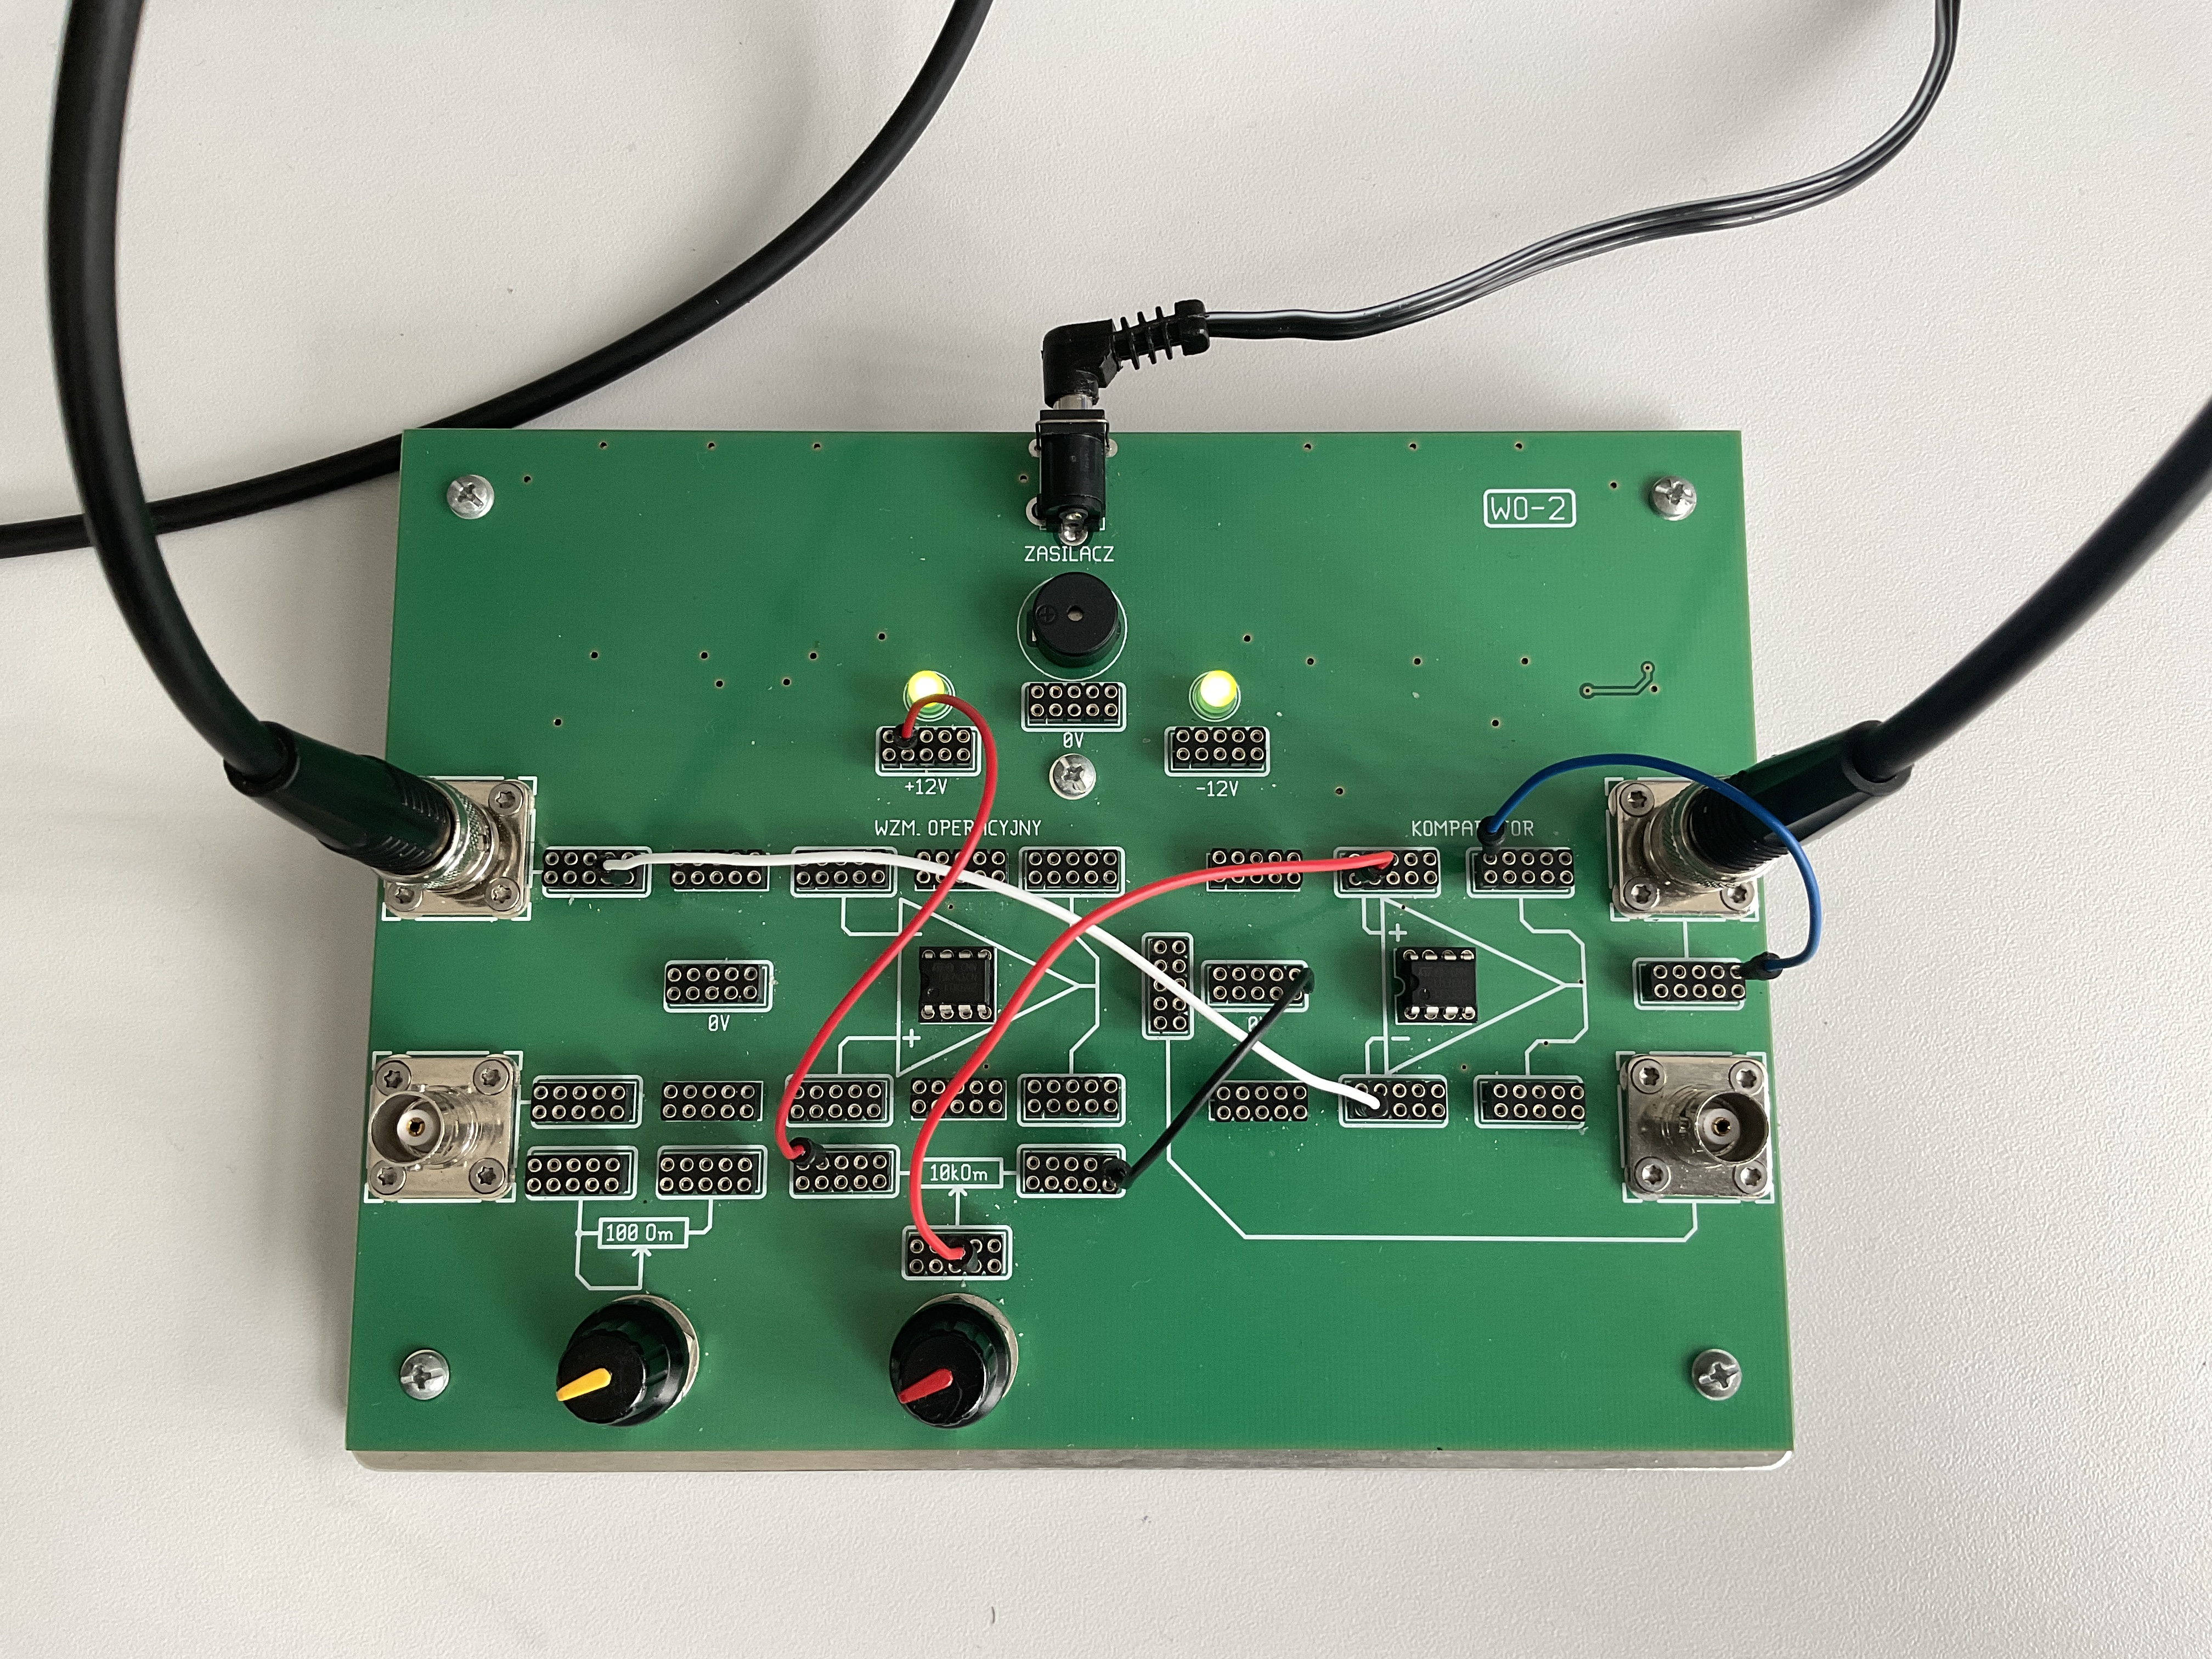
\includegraphics[width=16cm]{C10}
\centering
\captionsetup{labelformat=empty}
\caption{Zdjęcie 10: Układ zmontowany według schematu.}
\end{figure}

\newpage
Po zmontowaniu układu podałem na jego wejście sygnały z generatora o różnych kształtach i częstotliwościach. Obserwowałem przebiegi na wyjściu układu na oscyloskopie.

\begin{figure}[H]
\includegraphics[width=12cm]{A20}
\centering
\captionsetup{labelformat=empty}
\caption{Wykres 14: Fala sinusoidalna.}
\end{figure}

\begin{figure}[H]
\includegraphics[width=12cm]{A21}
\centering
\captionsetup{labelformat=empty}
\caption{Wykres 15: Fala trójkątna.}
\end{figure}

\begin{figure}[H]
\includegraphics[width=12cm]{A23}
\centering
\captionsetup{labelformat=empty}
\caption{Wykres 16: Fala sinusoidalna, potencjometr przestawiony na większą wartość.}
\end{figure}

Funkcją komparatora LM311 jest porównanie wartości na jego dwóch wejściach. Jeżeli w danej chwili napięcie na wejściu (-) jest wyższe niż na wejściu (+) na wyjściu komparatora pojawi się logiczna jedynka ($5 \ V$), w przeciwnym wypadku będzie tam logiczne zero ($0 \ V$). W układzie powyżej możliwe jest wybranie wartości do której komparator porównuje wejście poprzez ustawienie potencjometru.

\newpage
\paragraph{Notatki z zeszytu labolatoryjnego \\}
Poniżej załączam notatki z zeszytu laboratoryjnego.

\begin{figure}[H]
\includegraphics[scale=0.2]{B0}
\centering
\captionsetup{labelformat=empty}
\caption{}
\end{figure}

\begin{figure}[H]
\includegraphics[scale=0.2]{B1}
\centering
\captionsetup{labelformat=empty}
\caption{}
\end{figure}

\begin{figure}[H]
\includegraphics[scale=0.2]{B2}
\centering
\captionsetup{labelformat=empty}
\caption{}
\end{figure}

\begin{figure}[H]
\includegraphics[scale=0.2]{B3}
\centering
\captionsetup{labelformat=empty}
\caption{}
\end{figure}

\end{document}